% ****** Start of file apssamp.tex ******
%
%   This file is part of the APS files in the REVTeX 4.2 distribution.
%   Version 4.2a of REVTeX, December 2014
%
%   Copyright (c) 2014 The American Physical Society.
%
%   See the REVTeX 4 README file for restrictions and more information.
%
% TeX'ing this file requires that you have AMS-LaTeX 2.0 installed
% as well as the rest of the prerequisites for REVTeX 4.2
%
% See the REVTeX 4 README file
% It also requires running BibTeX. The commands are as follows:
%
%  1)  latex apssamp.tex
%  2)  bibtex apssamp
%  3)  latex apssamp.tex
%  4)  latex apssamp.tex
%
\documentclass[%
reprint,
%superscriptaddress,
%groupedaddress,
%unsortedaddress,
%runinaddress,
%frontmatterverbose, 
%preprint,
%preprintnumbers,
%nofootinbib,
%nobibnotes,
%bibnotes,
amsmath,amssymb,
aps,
%pra,
%prb,
%rmp,
%prstab,
%prstper,
%floatfix,
]{revtex4-2}

\usepackage{subfiles}
\usepackage{graphicx}% Include figure files
\usepackage{dcolumn}% Align table columns on decimal point
\usepackage{bm}% bold math
\usepackage{float}
\usepackage{mathtools}
\usepackage{xcolor}
\usepackage{physics}
\usepackage{dsfont}
\usepackage{tcolorbox}
\usepackage{float}
\usepackage{tensor}
\usepackage{hyperref}% add hypertext capabilities
\usepackage{subcaption}
%\usepackage[mathlines]{lineno}% Enable numbering of text and display math
%\linenumbers\relax % Commence numbering lines

%\usepackage[showframe,%Uncomment any one of the following lines to test 
%%scale=0.7, marginratio={1:1, 2:3}, ignoreall,% default settings
%%text={7in,10in},centering,
%%margin=1.5in,
%%total={6.5in,8.75in}, top=1.2in, left=0.9in, includefoot,
%%height=10in,a5paper,hmargin={3cm,0.8in},
%]{geometry}
\newcommand{\Hp}{\mathcal{H}}
\renewcommand{\thesection}{\arabic{section}}
\renewcommand{\thesubsection}{\thesection.\arabic{subsection}}
\renewcommand{\thesubsubsection}{\thesubsection.\arabic{subsubsection}}
\renewcommand{\figurename}{Fig.}
\renewcommand{\tablename}{Table}
\makeatletter
\renewcommand{\subsubsection}{%
	\@startsection
	{subsubsection}%
	{3}%
	{\z@}%
	{.8cm \@plus1ex \@minus .2ex}%
	{.5cm}%
	{\normalfont\small\centering}%
}
\makeatother
\renewcommand{\L}{\mathcal{L}}
\renewcommand{\O}{\mathcal{O}}
\newcommand{\f}[2]{\frac{#1}{#2}}
\newcommand{\p}{\partial}


\begin{document}
	
\title{Project 2}
\author{Edvard B. Rørnes}
\email{e.b.rornes@fys.uio.no}
\author{Isak O. Rukan}
\email{icrukan@uio.no}
\affiliation{Institute of Physics, University of Oslo,\\0371 Oslo,  Norway}
\date{\today}

\begin{abstract}
	In recent years, neural networks have become increasingly important for advancements in various scientific fields. In this report, we develop a program\footnote{\href{https://github.com/EdvardRornes/FYS-STK4155/tree/main/Project1}{Github}} that consists of both linear and logistic regression methods and a feed-forward neural network. In particular, the program implements gradient descent, stochastic gradient descent, and a simple feed-forward neural network with backpropagation. The neural network is evaluated against linear regression on the Franke function and against logistic regression using sklearn's breast cancer data, where it identifies malignant tumors. We explore three activation functions: Sigmoid, ReLU, and LeakyReLU. The analysis involves tuning the number of epochs, hidden nodes, and the hyperparameters $\lambda$ (regularization) and $\eta$ (learning rate) to optimal values. On the Franke function, our own implementation of the neural network achieved a peak $R^2$-score of $x$ and $y$ respectively. For the cancer data, the highest accuracies achieved with ReLU, , and Sigmoid activation functions were $97.9\%, 98.6\%$, and $97.9\%$, respectively, compared to $z\%$ for logistic regression. Notably, both the Sigmoid and LeakyReLU activation functions exhibited minimal sensitivity to variations in the hyperparameter $\lambda$ at optimal learning rates, whereas ReLU showed significant responsiveness. Overall, while LeakyReLU yielded the best performance across all tests, its improvement over the other activation functions was marginal when applied to the cancer dataset, but considerate on the Franke function. Additionally, the Sigmoid activation function was found to be appreciably slower than the ReLU variants.
\end{abstract}

\maketitle

\section{Introduction}
Over the last few years, machine learning and neural networks have become an increasingly important part of data analysis with an enormous range of applications. From image recognition to predictive analytics and scientific simulations, these techniques are reshaping the way the scientific community tackles complicated problems. The flexibility of neural networks in approximating complex, non-linear relationships has made them invaluable across diverse fields, such as biology, engineering, finance, physics etc. For just a few examples, see \cite{dawid2023modernapplicationsmachinelearning,thapar2023applicationsmachinelearningmodelling,mohammadi2022applicationsmachinelearninghealthcare}.

Neural networks are a powerful tool for handling large datasets where traditional modeling may fall short. This allows us to extract patterns and make accurate predictions. As the applications of these techniques continue to expand, so does the demand for a deeper understanding of their underlying principles and implementation details. Thus, we aim to investigate the foundational aspects of neural networks, explore various activation functions and learning algorithms, and study their effects on model performance. By doing so, we hope to develop a robust framework for applying neural networks effectively to complex real-world data.

The main goal of this project is understand the various techniques behind machines learning, and investigate they can be applied to the healthcare system, specifically in diagnosing malignant breast cancer tumors based on the tumor's several features based on the data from \texttt{sklearn}'s datasets \cite{sklearn}. We do this by testing the performance of a neural network by comparing it with logistic regression as we are working with discrete data. 

We begin by introducing the relevant background necessary to understand the implementations. Then we outline said implementations before discussing the results. We go over both linear and non-linear regression on the Franke function where performance issues in the implementation are easier to visualize. Finally the neural network and logistic regression are applied to the cancer data. 

\section{Methods}
In this section we present the various methods used in this report. 

\subsection{Linear Regression}
As discussed in a previous project \cite{project1}, linear regression is the simplest method for fitting a continuous given a data set. The data set is approximated by $\bm y=\bm X\bm\beta$ and the $\beta$ coefficients are found by minimizing the cost function. For this project we consider the two regression methods:
\begin{align}
	C_\text{OLS}(\bm\beta)&=\frac{2}{n}(\bm y-\bm X\bm\beta)^2,\\
	C_\text{Ridge}(\bm\beta)&=C_\text{OLS}(\bm\beta)+\lambda||\bm\beta||_2^2.
\end{align}
We then insist that the derivative of these w.r.t. $\bm\beta$ is $0$, and choose the resulting $\beta$ coefficients as out model. Doing this we arrive at:
\begin{align}
	\bm\beta_\text{OLS}&=(\bm X^T\bm X)^{-1}\bm X^T\bm y,\\
	\bm\beta_\text{Ridge}&=(\bm X^T\bm X+\lambda \bm I)^{-1}\bm X^T\bm y.
\end{align}

\subsection{Regularization Terms}
Regularization is a technique to prevent overfitting by adding a penalty to the cost function that discourages complex models. Overfitting occurs when a model learns the noise in the training data rather than the underlying patterns, leading to poor generalization on unseen data. In the context of neural networks, regularization plays a critical role, especially when working with architectures that have many parameters.

The two common regularization methods that we inspected previously are Ridge and Lasso regularization. In this project, we will only be considering Ridge regularization, where the cost function is given by
\begin{align}
	C_\text{Ridge}(\bm \beta)=C_\text{OLS}(\bm\beta)+\lambda\bm\beta_2^2,
\end{align}
where \(C_\text{OLS}(\bm\beta)\) is the ordinary least squares cost function, \(\bm\beta\) represents the model parameters, and the hyperparameter \(\lambda\) controls the magnitude of the penalty to large coefficients. For more details on regularization in linear regression, see \cite{project1}.

In the context of neural networks, regularization techniques are crucial for controlling model complexity and improving generalization. Ridge regularization can be implemented in neural networks by applying L2 regularization to the weights of the network. This approach adds the penalty term \( \lambda \|\mathbf{W}\|_2^2 \) to the loss function, where \( \mathbf{W} \) is the weight matrix of the neural network. The modified cost function for a neural network with L2 regularization becomes
\begin{align}
	C_{\text{NN}}=C_{\text{loss}}+\lambda \|\mathbf{W}\|_2^2,
\end{align}
where \( C_{\text{loss}} \) will be the MSE for regression tasks and cross-entropy loss for classification tasks.

Incorporating regularization in neural networks offers several important benefits. Firstly, L2 regularization effectively applies weight decay, which shrinks the weights during training and helps prevent the model from becoming overly complex. This leads to smoother decision boundaries and reduces the risk of overfitting, allowing the model to generalize better to unseen data. Secondly, regularized models tend to exhibit increased robustness to variations in the data, as the penalty encourages the learning of simpler models that do not fit the noise in the training set. Lastly, by tuning the hyperparameter \( \lambda \), practitioners can effectively control the model's complexity, striking a balance between bias and variance and tailoring the model to the specific problem at hand. Overall, these advantages highlight the critical role that regularization plays in developing neural networks that perform well in real-world applications.

Overall, incorporating regularization terms such as Ridge regularization in the training of neural networks is essential for developing models that generalize well to new, unseen data. 


\subsection{Logistic Regression}
Whilst linear regression is quite successful in fitting continuous data such as terrain data, when the output is supposed to be discrete it fails. Linear regression predicts values across a continuous spectrum, resulting in predictions outside the range of valid class labels, such as giving negative probabilities. Logistic regression on the other hand is specifically designed for binary classification problems, and is thus ideal when dealing with discrete outcomes. 

Logistic regression models the probability that a given input belongs to a particular class, typically using the sigmoid function to map any real-valued number to a value between 0 and 1. Given an input vector $\bm X$ and weights $\bm\beta$, logistic regression predicts the probability of the class as:
\begin{align}
	P(y=1|\bm X)=\sigma(\bm X\bm\beta)=\frac{1}{1+e^{-\bm X\bm\beta}}
\end{align}
where $\sigma$ represents the sigmoid function. To find optimal weights, logistic regression minimizes the cross-entropy cost function:
\begin{align}
	C(\bm\beta)=-\frac1n\sum_{i=1}^n\left(y_i \ln(\hat y_i)+(1-y_i)\ln(1-\hat y_i) \right)
\end{align}
where $y_i$ is the class label and $\hat{y}_i$ is the predicted probability for sample $i$. To penalize overfitting, and regularization term may be added to \(C(\bm\beta)\). This terms adds a penalty for large weights, trying to keep the weights (relatively) small. Adding the \(\ell^2\) regularization term results in 
\begin{align}
	C(\bm\beta)=-\frac1n\sum_{i=1}^n\left(y_i \ln(\hat y_i)+(1-y_i)\ln(1-\hat y_i) \right) + \lambda\sum\limits_{i=1}^{n}w_{j}^{2}.
\end{align}

\subsection{Resampling Methods}
Resampling methods are used to estimate the accuracy of predictive models by splitting the data into training and testing sets or by generating multiple datasets. Common techniques include cross-validation and bootstrapping. In cross-validation, the data is split into $k$ folds, and the model is trained on $k-1$ folds and tested on the remaining fold. This process is repeated $k$ times, and the average accuracy is computed. Bootstrapping involves sampling with replacement from the dataset to create multiple training sets. These methods help assess model stability and generalizability on unseen data.

\subsection{Gradient Descent}
Gradient descent (GD) is an essential optimization algorithm in machine learning, commonly used to minimize cost functions by adjusting model parameters iteratively. Given model parameters $\theta$ and a cost function $C(\theta)$, the GD update rule adjusts parameters in the opposite direction of the gradient:
\begin{align}
	\theta_i^{(j+1)}=\theta_i^{(j)}-\eta\pdv{C}{\theta_i}
\end{align}
where $\eta$ is the learning rate. Batch gradient descent (BGD) calculates the gradient over the entire dataset:
\begin{align}
	\theta^{(j+1)}=\theta^{(j)}-\eta\nabla_\theta C
\end{align}
BGD is computationally expensive for large datasets but provides smooth convergence toward the minimum.

\subsection{Stochastic Gradient Descent}
Stochastic Gradient Descent (SGD) is a variation of gradient descent where each parameter update is performed on a single data point or a small batch. The update rule for SGD is:
\[
\theta_i^{(j+1)} = \theta_i^{(j)} - \eta \pdv{C^{(i)}}{\theta_i}
\]
where $C^{(i)}$ is the cost function evaluated at a single data point $i$. While SGD introduces noise in the updates, it often converges faster for large datasets and helps escape local minima, making it ideal for training neural networks.

\subsection{Neural Networks}
Neural networks are computational models inspired by the human brain, designed to recognize patterns and relationships within data. They consist of layers of interconnected neurons or nodes, where each neuron applies a transformation to the input data. In each layer, neurons take a weighted sum of inputs, apply an activation function to introduce non-linearity, and pass the result to the next layer. The final layer produces the output, serving as the network’s prediction.

\subsubsection{Feed Forward Neural Networks}
Feed-forward neural networks (FFNNs) are the simplest type of neural network, where data flows forward from input to output without forming cycles. These networks contain one or more hidden layers that apply an activation function to capture complex, nonlinear patterns in the data. The training process adjusts the weights of each connection to minimize a cost function, typically using gradient descent.

\subsubsection{Activation Functions}
Activation functions play a critical role in neural networks by introducing non-linearity, which enables the network to approximate more complex functions beyond simple linear mappings. In this project, we use three different activation functions: sigmoid, tanh, ReLU, and Leaky ReLU. Each function has different properties that can impact training performance and convergence.
\begin{itemize}
	\item The sigmoid function, suitable for binary classification, takes an input $z\in\mathbb{R}$ and outputs a value in the range $(0,1)$. This makes it useful for probabilistic interpretations. As mentioned prior, it is given by:
	\begin{align} 
		\sigma(z)=\frac{1}{1+e^{-z}}.
	\end{align}
	\item The ReLU (Rectified Linear Unit) function activates only positive values: 
	\begin{align} 
		R(z)=
		\begin{cases}
			0 & \text{if }z\leq0\\z&\text{if }z>0
		\end{cases}.
	\end{align}
	This reduces the number of calculations that the network has to perform and can speed up the training.
	\item The Leaky ReLU (LReLU) function is a variation of ReLU that allows a small gradient when $z\leq0$. This can help mitigate a known issue known as ``dying ReLU'' where neurons become inactive due to consistently recieving negative inputs., helping to mitigate issues with inactive neurons. It is given by:
	\begin{align} 
		LR(z)=
		\begin{cases} 
			az&\text{if }z\leq0\\z&\text{if }z> 0 
		\end{cases} 
	\end{align}
	where $a$ is some small number. In this project we consider only $a=0.01$.
\end{itemize}
By selecting appropriate activation functions for each layer, FFNNs can effectively capture complex data patterns, enhancing model performance.

\subsubsection{Backpropagation}
Backpropagation is the key algorithm for training neural networks by optimizing weights to minimize the cost function. It works by propagating the error backward from the output layer to the input layers, computing gradients for each weight based on the error. These gradients are then used to update the weights, enabling the network to learn from its errors and make more accurate predictions over time.

\section{Implementation}
(Write about your implementation Isak)

Further, the Feedforward Neural Network (FFNN) was implemented to be able to analyze both the Franke function and the breast cancer data. The FFNN is structured with an input layer, one or more hidden layers, and an output layer, with each layer utilizing an activation function, and currently only supports the Adam optimizer. The architecture is defined by specifying the input size, the number of neurons in hidden layers, and the output size. In the case of the Franke function, the input layer is size 2, one for $x$ and one for $y$, whilst for the breast cancer data the input layer corresponds to the number of features, i.e. $30$, which corresponds to several properties of the tumor, such as circumference, density etc. 

We tested out various different ways of layering the hidden layers. In the end, for the Franke function, we settled with using a pyramid-like architecture for the hidden layers $[4,8,16,32,16,8,4,2]$ whilst for the breast cancer data we used $[15,30,15,8,4,2]$. These were decided on based on the size of both the input and output, where the latter is $1$ in both cases. The weights and biases are initialized using random values scaled by the number of input neurons, which aids in faster convergence during training. The network supports ReLU, Sigmoid, and Leaky ReLU as activation functions. The forward propagation computes the output of the network by applying the activation function to the weighted sum of inputs at each layer. The backward propagation algorithm updates the weights and biases using gradient descent, where the mean squared error serves as the loss function. We implement regularization techniques to mitigate overfitting.

The training process includes splitting the data into training and test sets, followed by iterating through a specified number of epochs, during which the network adjusts its weights to minimize the error. The test size used throughout is $25\%$. After training, the network can predict outputs for new data, allowing for evaluation against known values from the Franke function. The overall performance of the model is assessed using MSE and accuracy for Franke and cancer data respectively.


\section{Results \& Discussion}
We represent the results and compare the various methods. The larger plots have been placed in Appendix \ref{Appendix:A} to preserve space for the sake of readability.

\subsection{Franke}
The results for the MSE and $R^2$ as a function of the learning rate $\eta$ with 1000 epochs with our own FFNN with different activation functions and keras NN with the sigmoid activation function are given in Fig. \ref{fig:NN_Franke_LR_1000}. In this particular plot we are not using any regularization terms. The reason for this is simply due to \texttt{keras} being very slow, but we still wanted to include it as a reference. The optimal learning rates for $\lambda=0$ can easily be read off this plot.
\begin{figure}[ht!]
	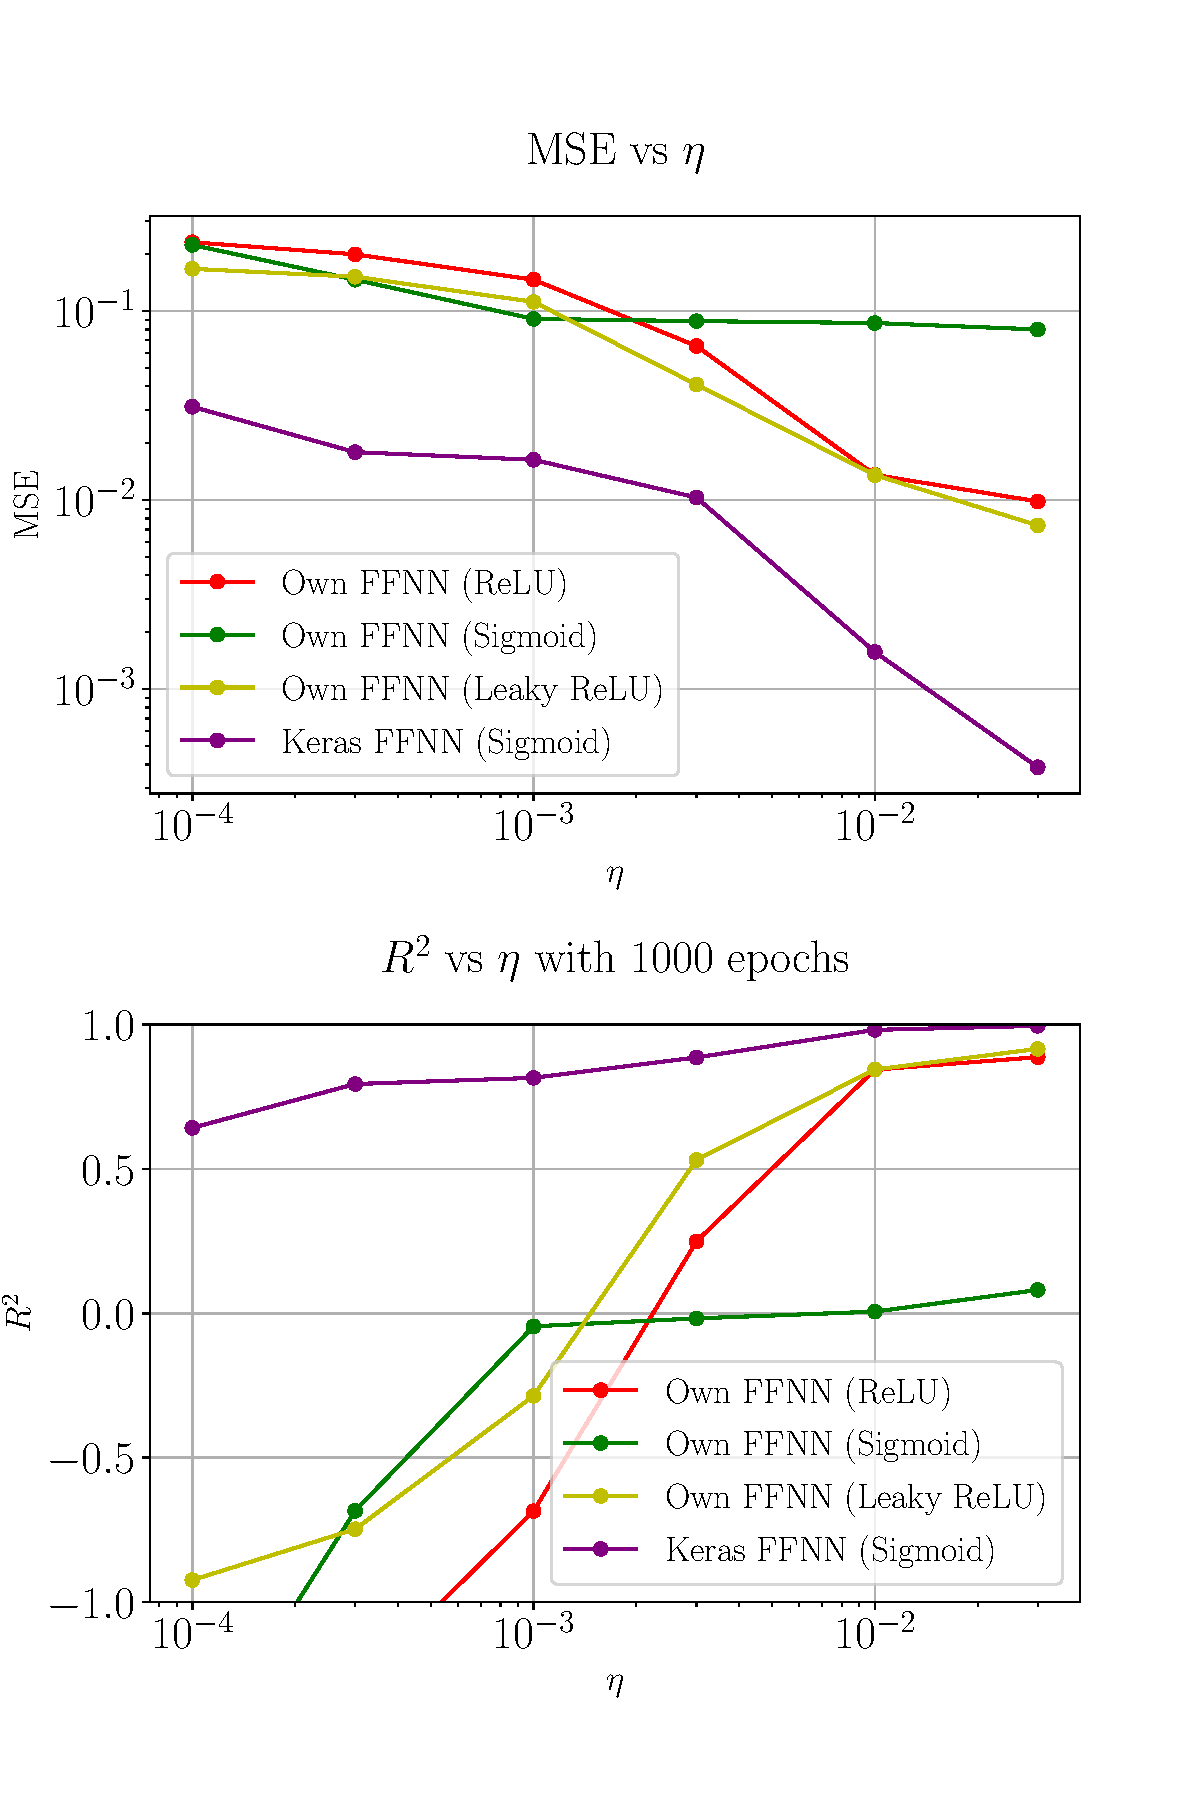
\includegraphics[width=0.5\textwidth]{Python/Figures/NN_MSE_R2_Franke_LearningRate_Epochs1000.pdf}
	\caption{MSE and $R^2$ regression results for the FFNN as a function of $\eta$ with 1000 epochs.}
	\label{fig:NN_Franke_LR_1000}
\end{figure}

Further we used the result for the best learning rate to plot the MSE after each epoch, given in Fig. \ref{fig:NN_Franke_Epochs}. As expected, all activation functions perform poorly on low epochs, and gradually improve as you go along. At the end, all seem to achieve a relatively good MSE as the number of epochs increase.

Overall these metrics seem to imply that ReLU and LReLU are outperforming \texttt{keras}, but when explicitly plotting the predictions this does not seem to be the case, as can be seen in Fig. \ref{fig:3D_Franke}. Note that this plotted prediction is a rerun with the best parameters for each activation type. Thus their performance being worse here compared to \texttt{keras} may simply be due to large variation from one run to another in our implementation.
\begin{figure}[ht!]
	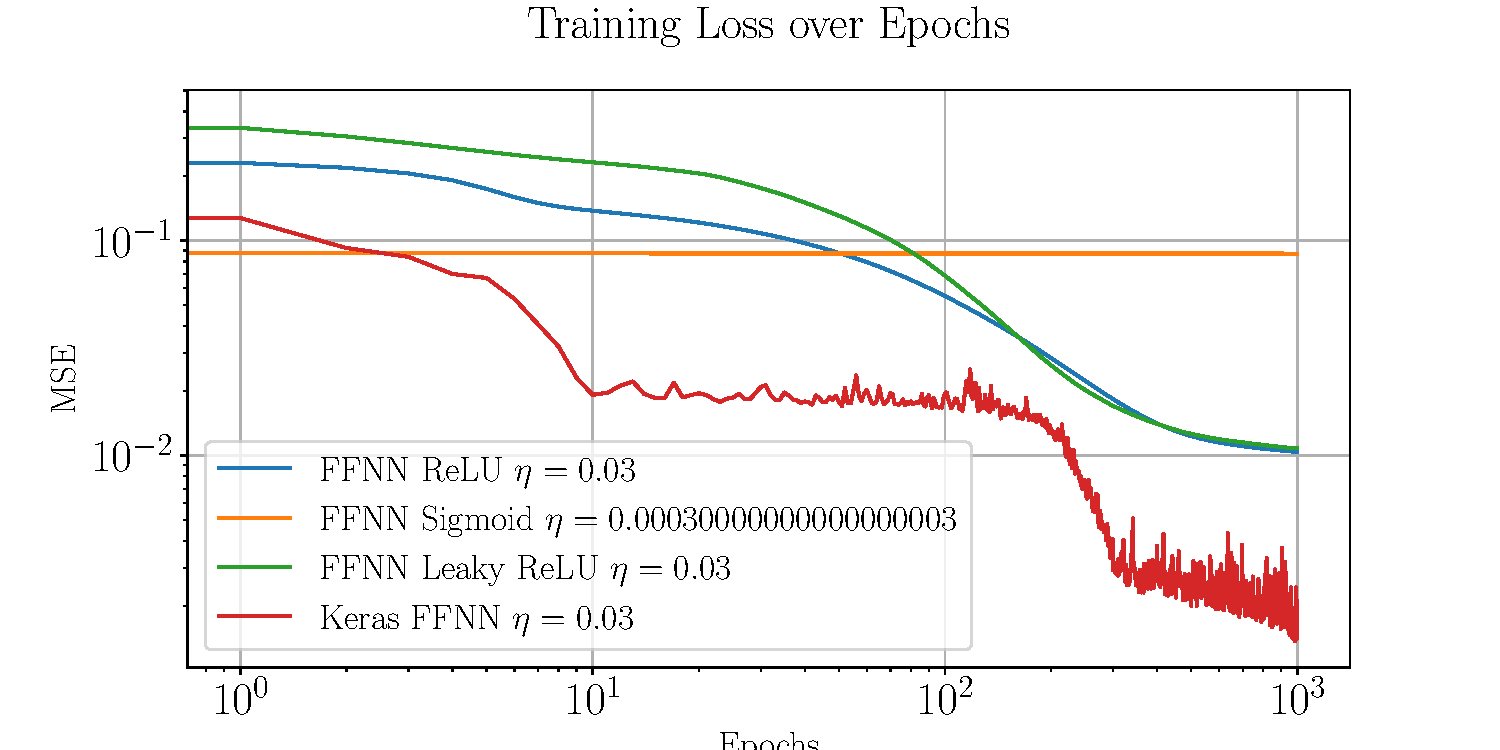
\includegraphics[width=0.5\textwidth]{Python/Figures/NN_MSE_Franke_Epoch.pdf}
	\caption{The MSE regression results for the FFNN as a function of number of epochs for ReLU, LReLU, Sigmoid and keras.}
	\label{fig:NN_Franke_Epochs}
\end{figure}

We then did the above again, but now with a regularization parameter $\lambda$ and excluded \texttt{keras} due to time constraints. The MSE for various combinations of $\eta$ and $\lambda$ are given in Fig. \ref{fig:FFNN_Franke_heatmaps}. The best results from here are then picked to once again plot the MSE over epochs given in Fig. \ref{fig:best_MSE_Franke_Epochs} and another 3D plot to visualize the results in Fig. \ref{fig:NN_noKeras_3D_Franke_Epochs250}. Clearly the sigmoid activation function performs worse overall, whilst ReLU and LReLU have a close competition between them. The convergence is much faster here, and we same performance with ReLU and LReLU after only $50$ epochs. The sigmoid function converges much slower, but this is due to it being suited for binary classification and not regression. The much faster convergence does suggest that the regularization parameter is improving our performance significantly.
\begin{figure}[ht!]
	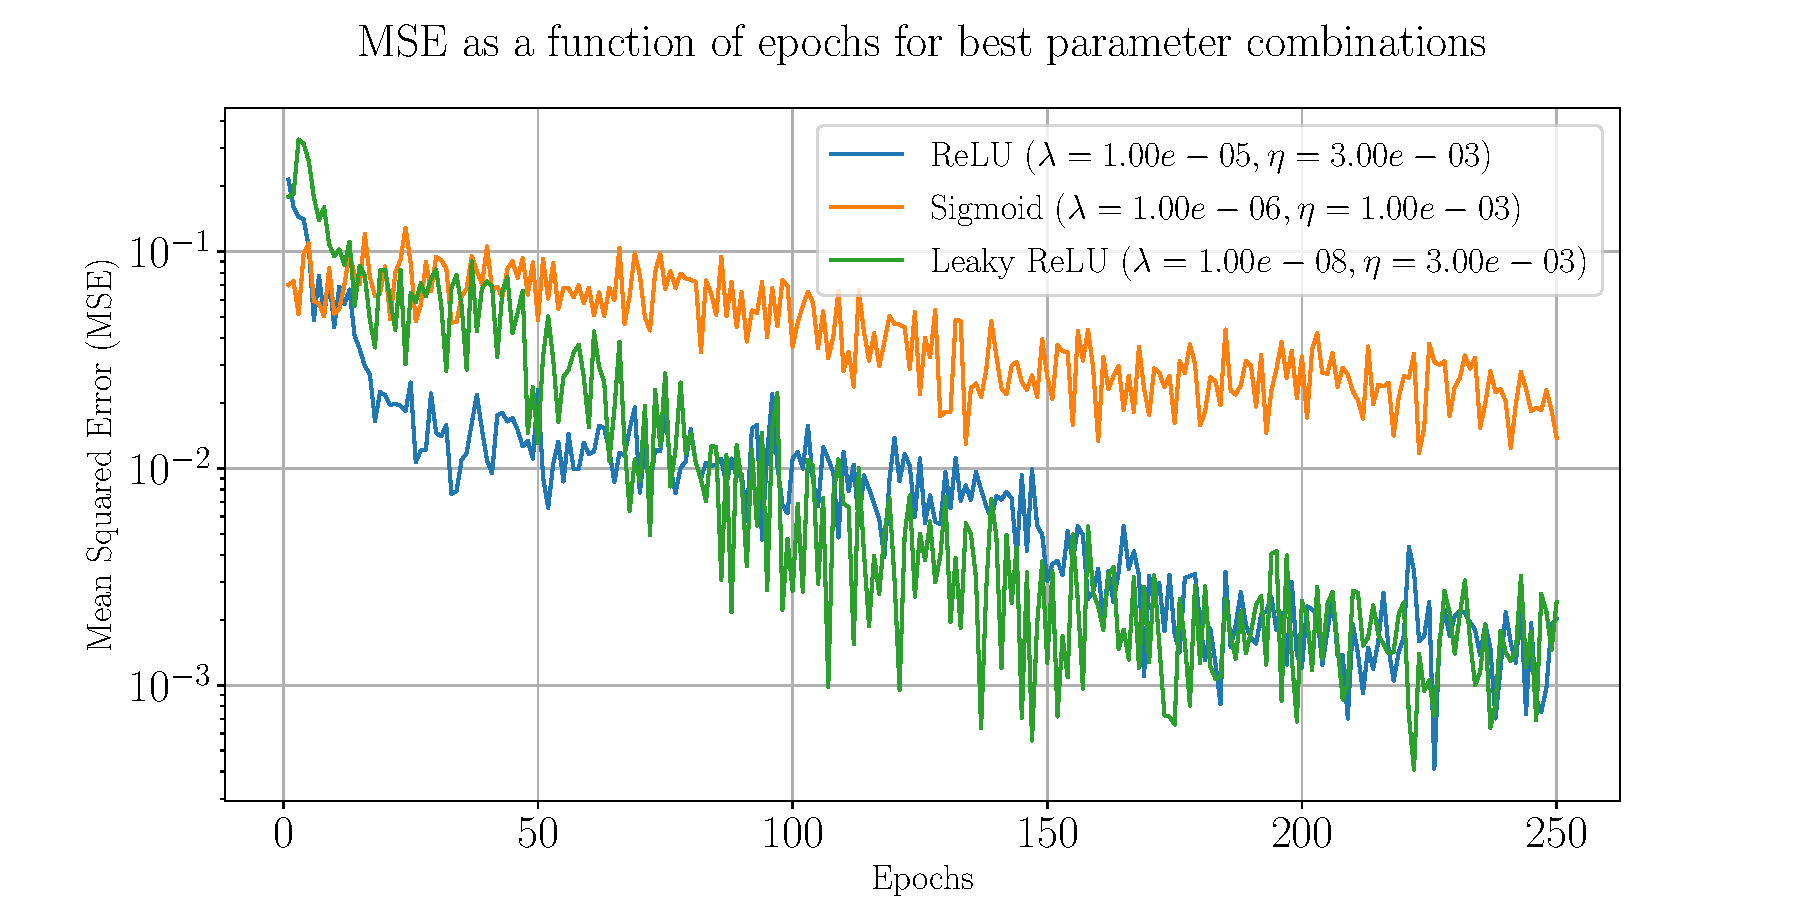
\includegraphics[width=0.5\textwidth]{Python/Figures/Best_MSE_vs_Epochs.pdf}
	\caption{The MSE regression results for the FFNN as a function of number of epochs for ReLU, LReLU, Sigmoid with the best performing combination of $\lambda$ and $\eta$.}
	\label{fig:best_MSE_Franke_Epochs}
\end{figure}


\subsection{Cancer Data}
The accuracy for logistic regression and our own FFNN for the three different activation functions and for different values of $\eta$ and $\lambda$ are given in Figs. \ref{fig:LogReg} and \ref{fig:FFNN_cancer_heatmaps} respectively.

\section{Conclusion}
On the Franke function, we found that Sigmoid is not overly sensitive to changes in the learning rate and hyperparameter $\lambda$, but also struggles to get good results. On the other hand ReLU has the ability to get great results, but only for very specific combinations of $\eta$ and $\lambda$. LReLU seems to be the best of both worlds, being relatively insensitive to getting the exact right combination of $\eta$ and $\lambda$, whilst still managing to obtain very good MSE scores like ReLU.  For logistic regression our FFNN performs quite well, approaching $98\%$ accuracy with certain parameter combinations.

A step forward would for example be testing out different values of $a$ in LReLU and seeing whether it may achieve a higher level of performance. Thoroughly testing out other optimizers such as Adagrad and RMSprop for the FFNN may also yield benefits, but due to time constraints we did not implement this properly. 

% Bibliography
\bibliographystyle{JHEP}
\bibliography{project2}

\appendix
\section{Large Figures}
\label{Appendix:A}

\begin{figure*}
	\begin{subfigure}{0.4353\textwidth}
		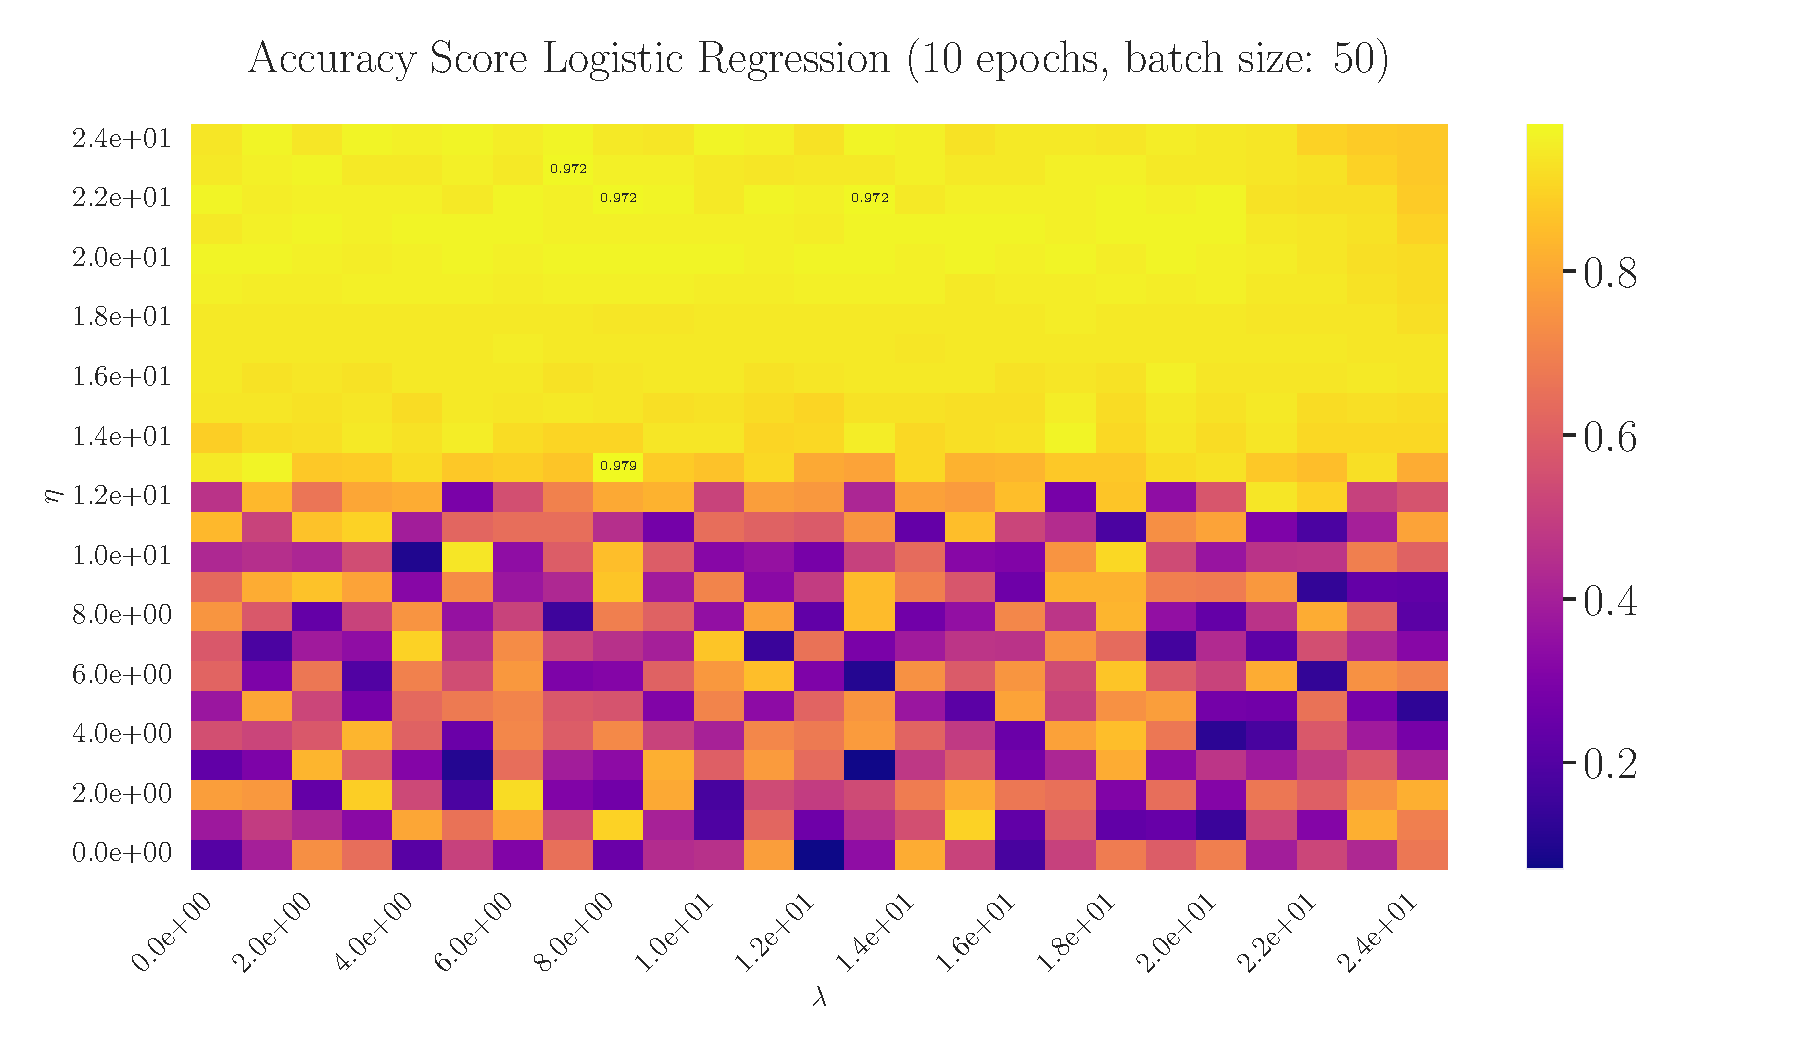
\includegraphics[width=\textwidth]{Python/Figures/LogReg25x25_epoch10_batchS50.pdf}
		\caption{ReLU}
		\label{fig:LogReg25x25_epoch10_bacthS50}
	\end{subfigure}
	\hfill
	\begin{subfigure}{0.4353\textwidth}
		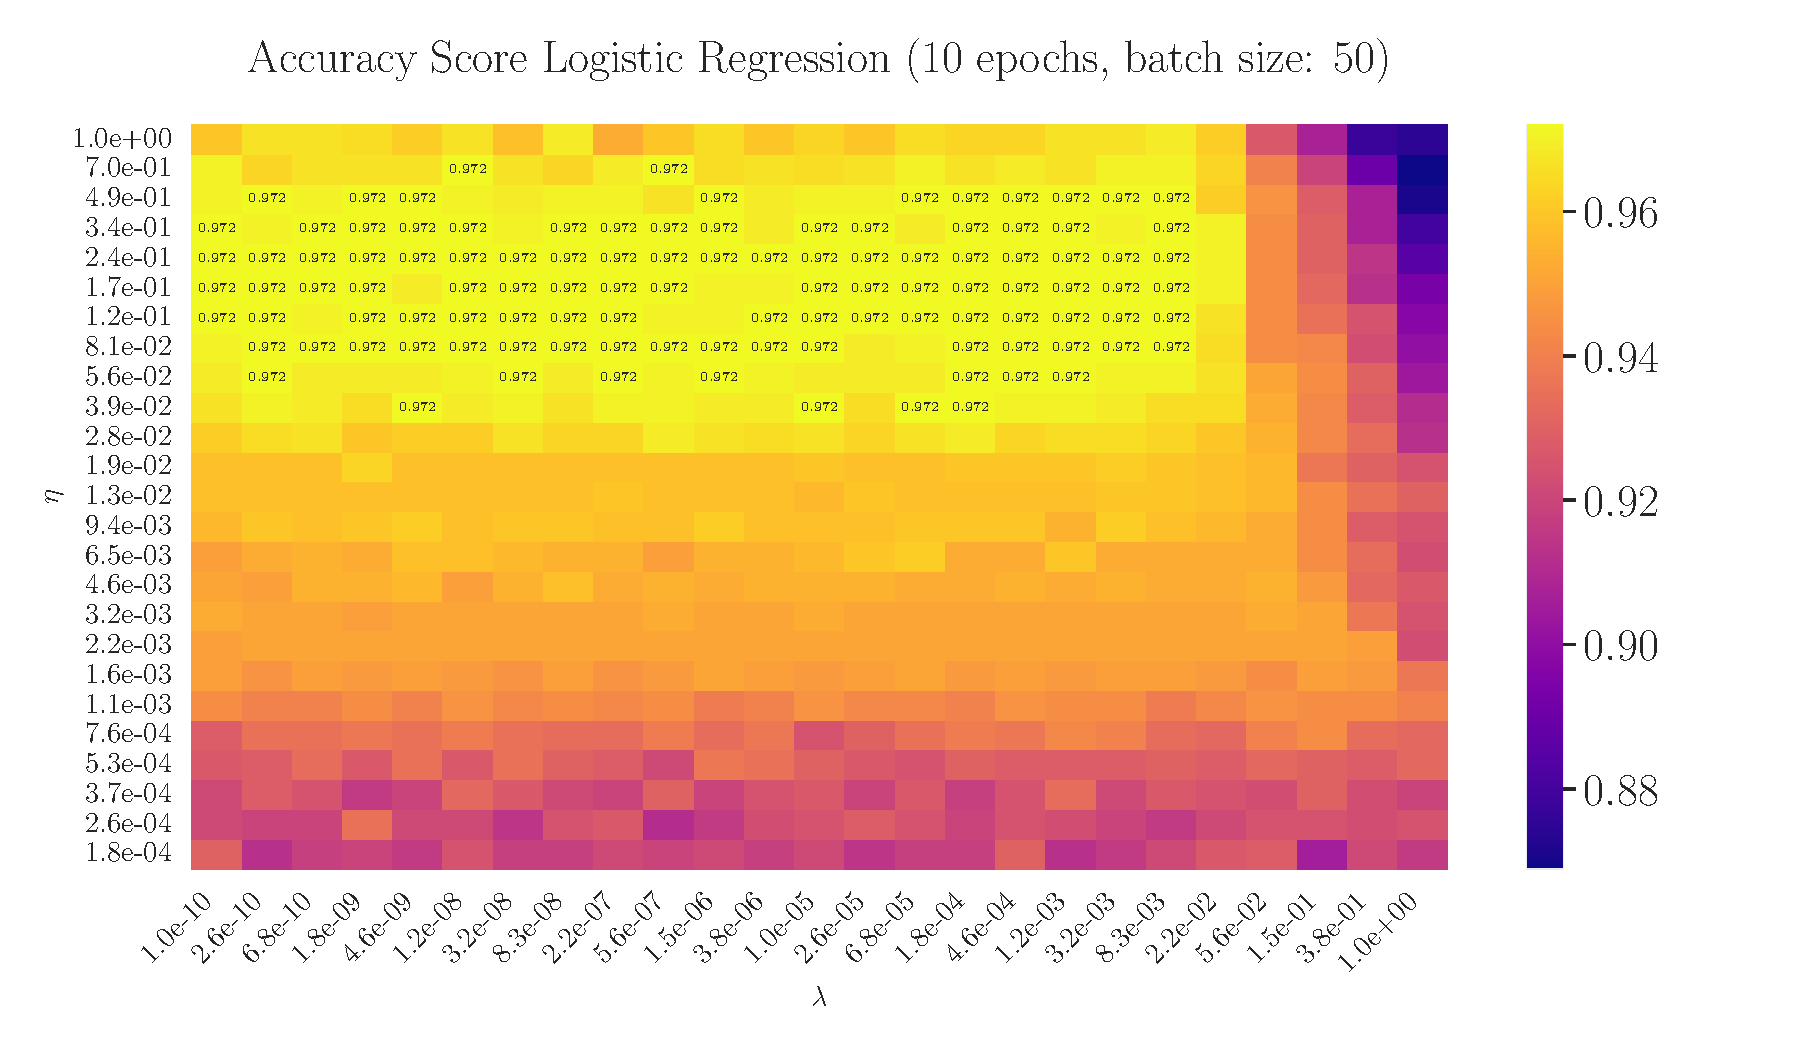
\includegraphics[width=\textwidth]{Python/Figures/LogReg25x25_epoch10_batchS50_zoomed.pdf}
		\caption{LReLU}
		\label{fig:LogReg25x25_epoch10_bacthS50_zoomed}
	\end{subfigure}
	\hfill\newline
	\begin{subfigure}{0.4353\textwidth}
		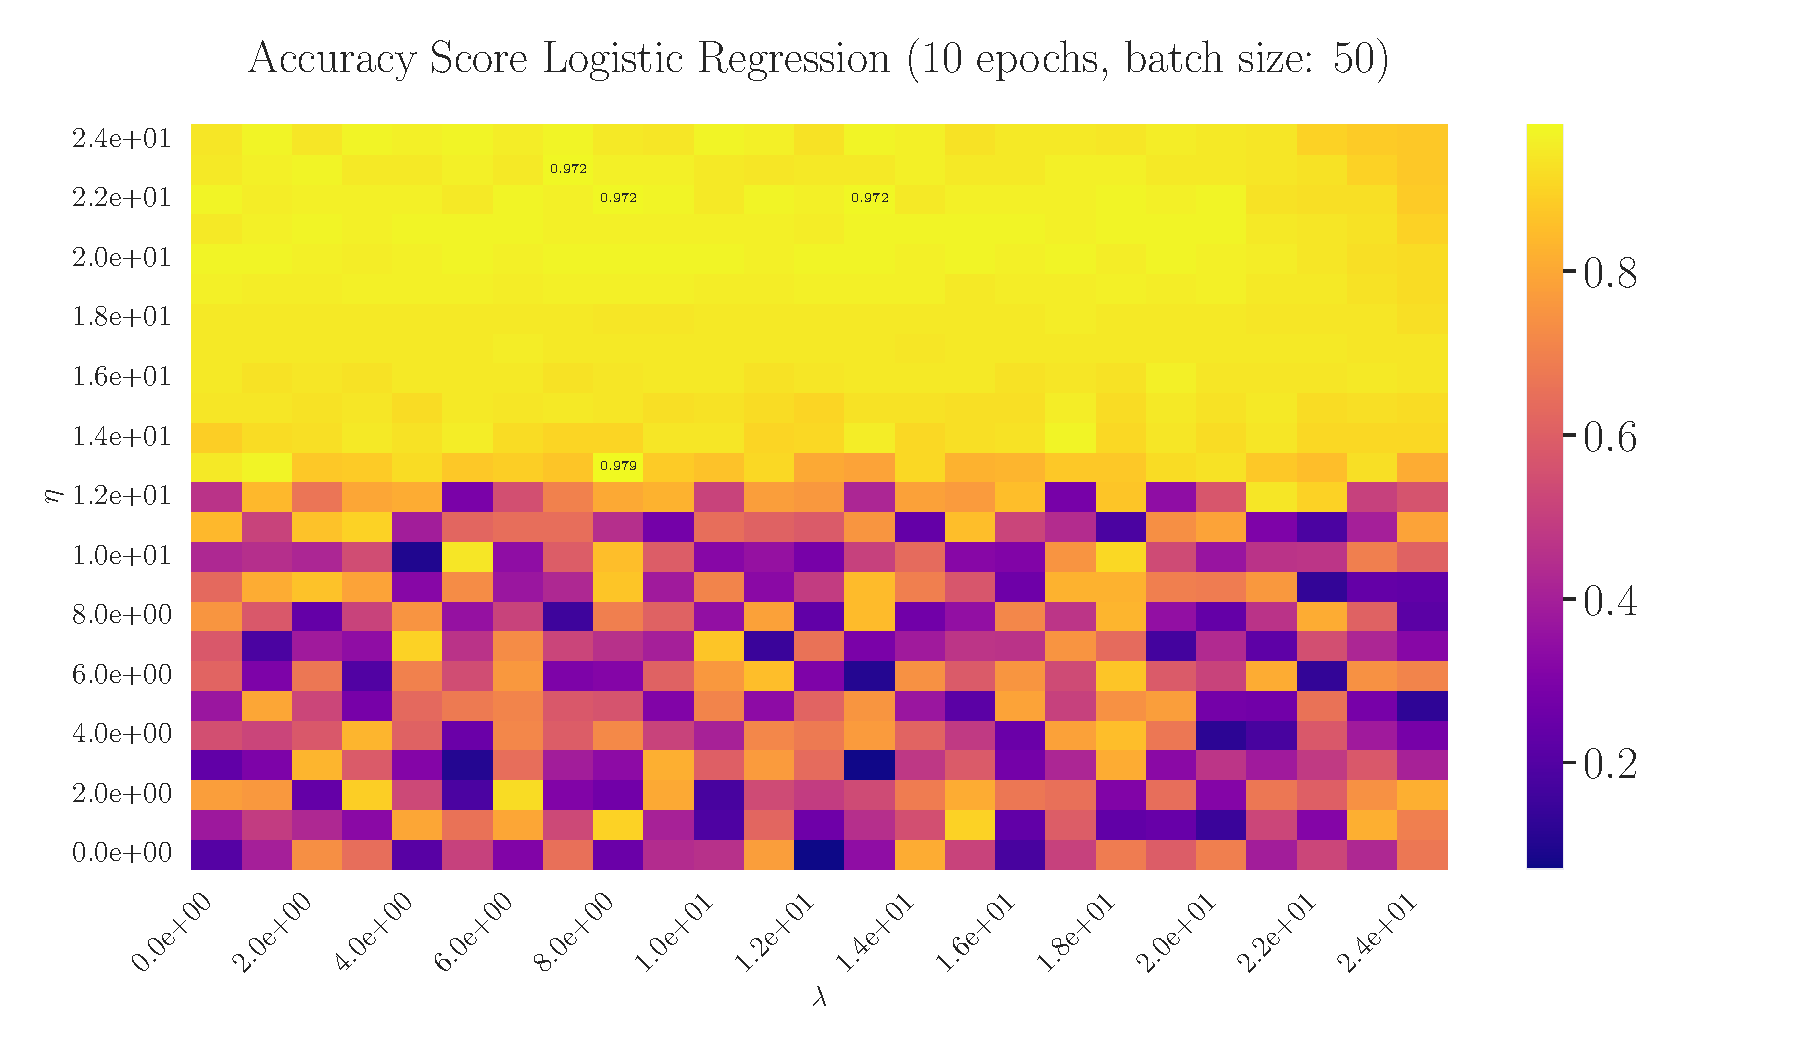
\includegraphics[width=\textwidth]{Python/Figures/LogReg25x25_epoch10_batchS50.pdf}
		\caption{Sigmoid}
		\label{fig:LogReg25x25_epoch100_bacthS50}
	\end{subfigure}
	\hfill
	\begin{subfigure}{0.4353\textwidth}
		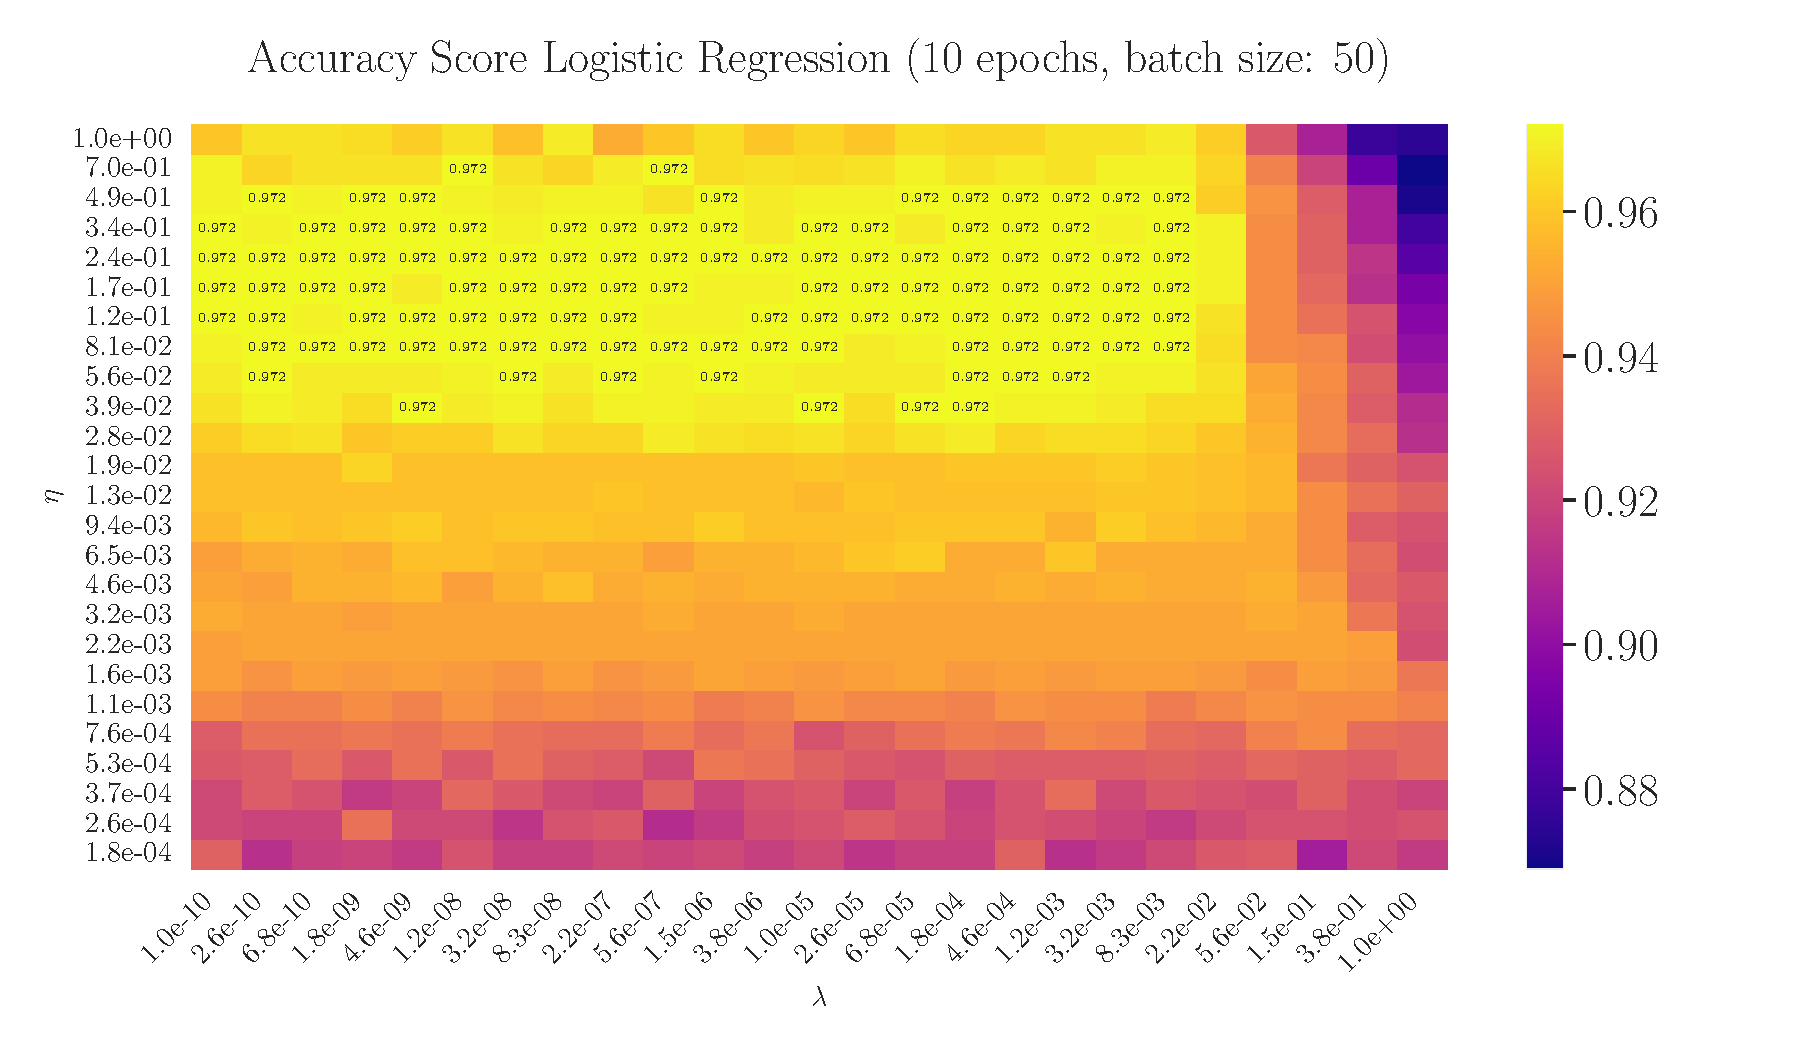
\includegraphics[width=\textwidth]{Python/Figures/LogReg25x25_epoch10_batchS50_zoomed.pdf}
		\caption{LReLU}
		\label{fig:LogReg25x25_epoch100_bacthS50_zoomed}
	\end{subfigure}
	\caption{Accuracy score for logistic regression, for number of epochs \(N=10\) (left), \(N=100\) (right). The figures to the right are zoomed in versions of the ones to the left.}
	\label{fig:LogReg}
\end{figure*}

\begin{figure*}[ht!]
\begin{subfigure}[b]{0.49\textwidth}
	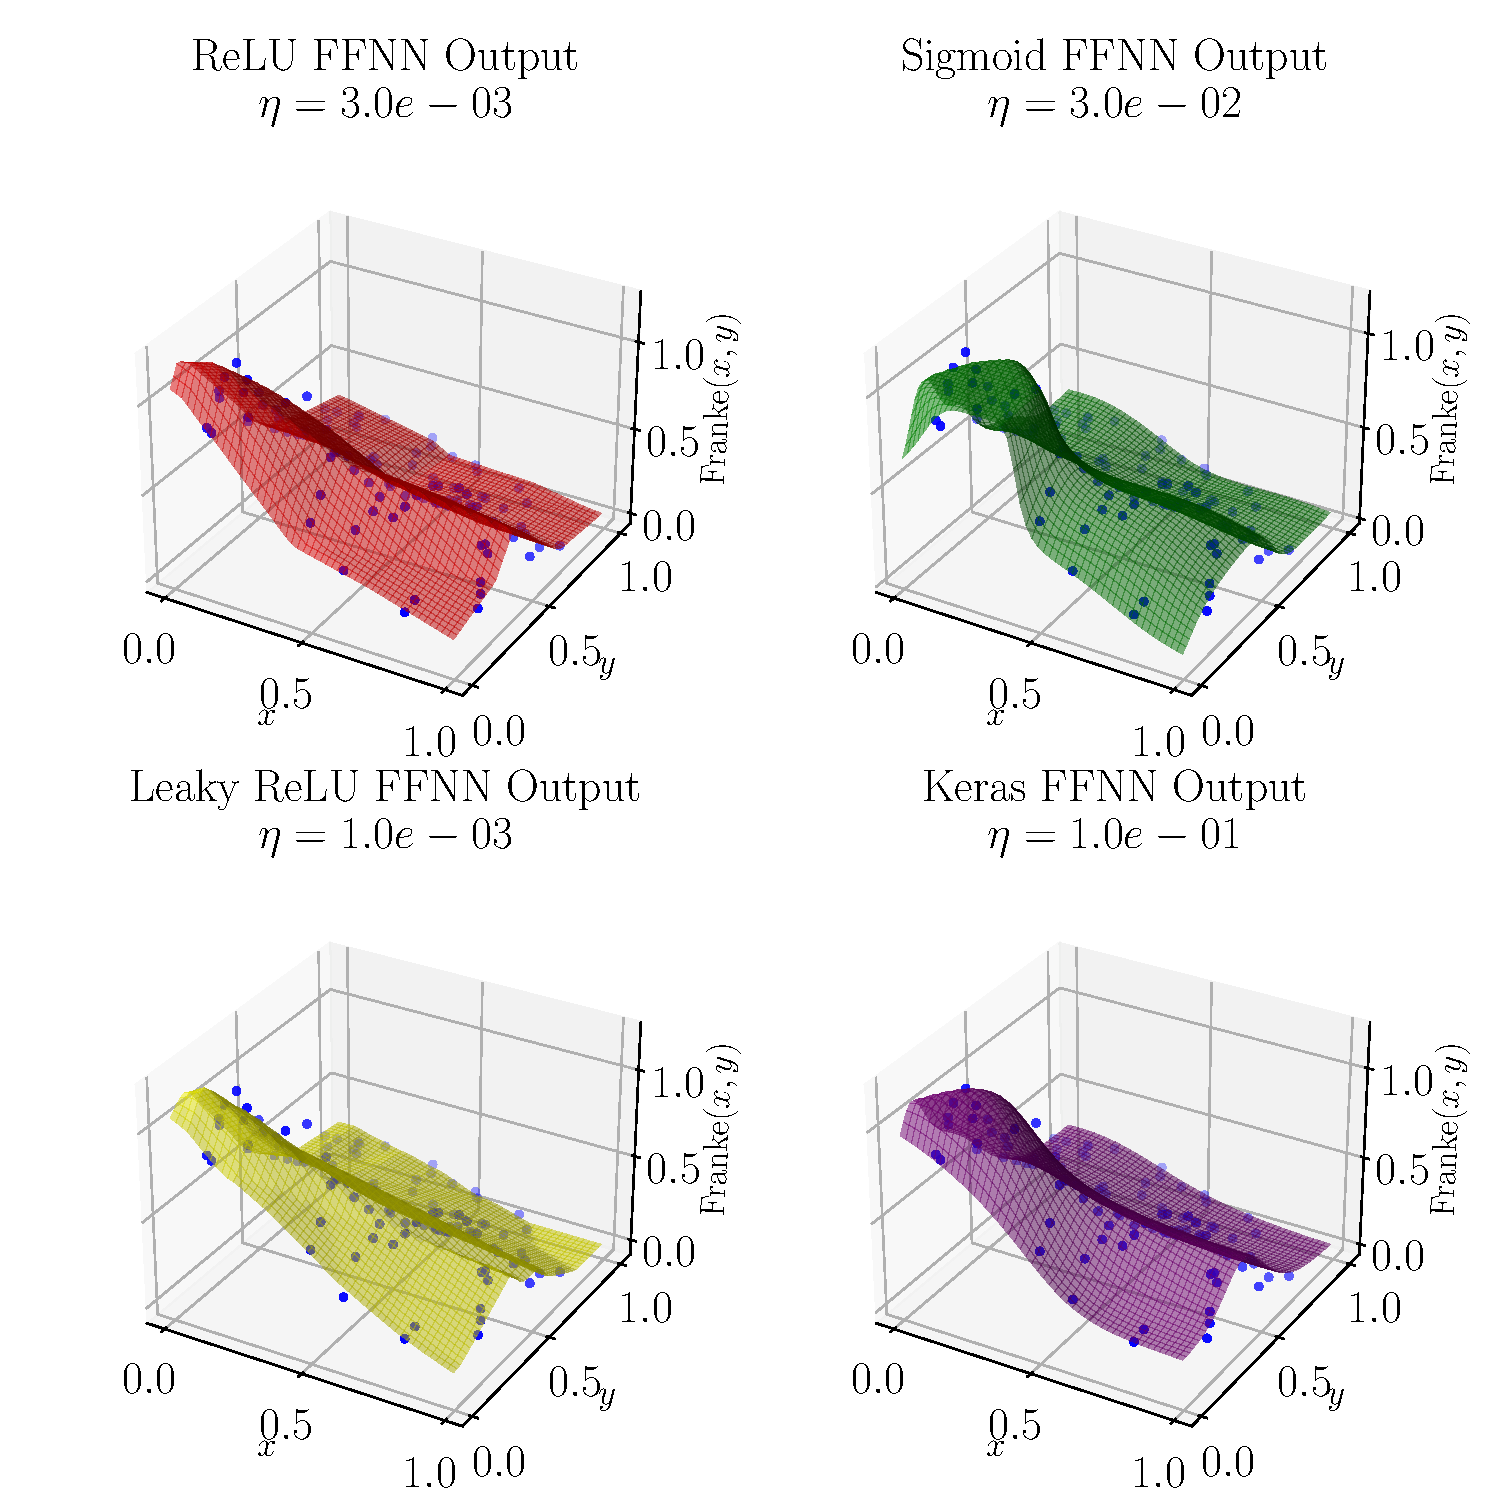
\includegraphics[width=\textwidth]{Python/Figures/NN_3D_Predict_Franke_Epochs1000.pdf}
	\caption{3D plots for best $\eta$ with $1000$ epochs. The blue dots correspond to the sampled points from the Franke function with $100$ total samples.}
	\label{fig:3D_Franke}
\end{subfigure}
\hfill
\begin{subfigure}[b]{0.49\textwidth}
	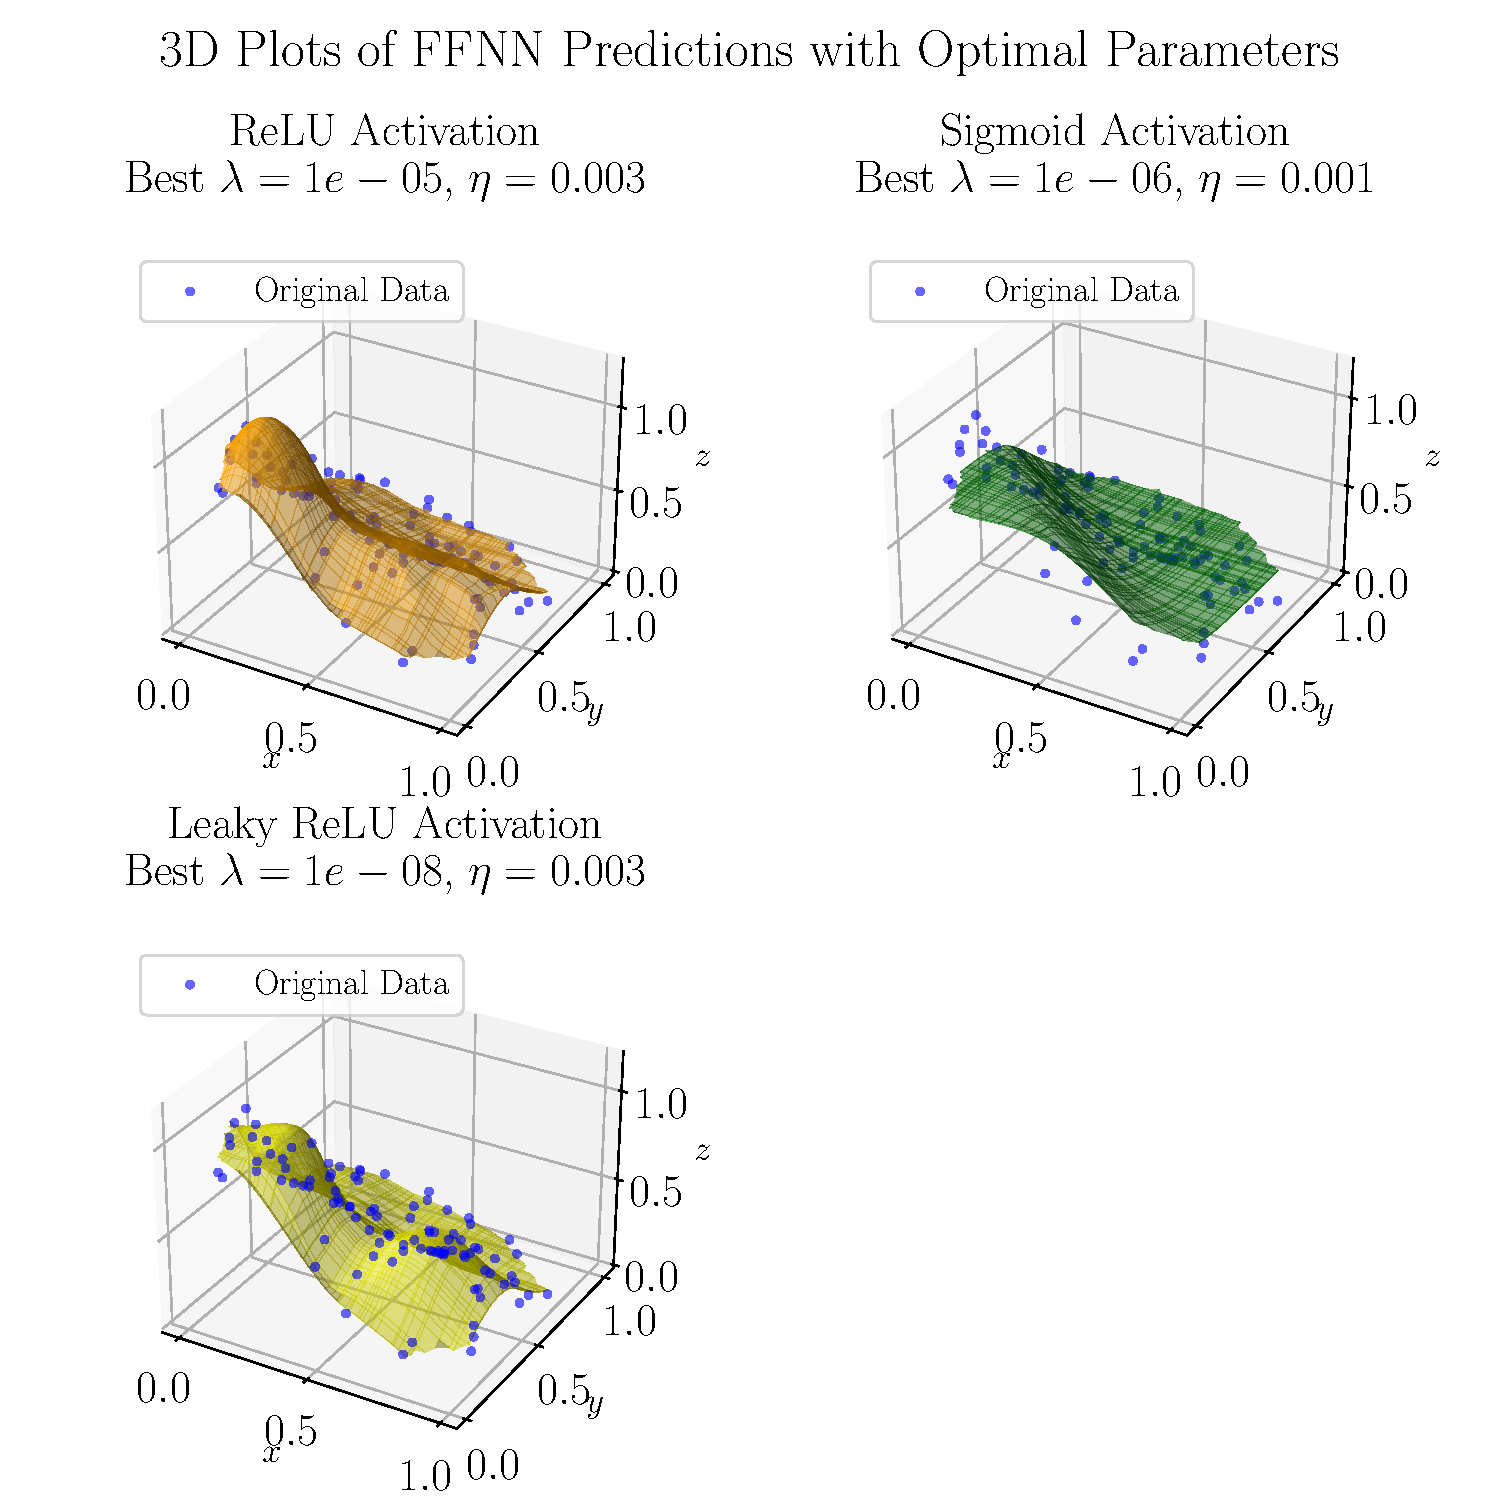
\includegraphics[width=\textwidth]{Python/Figures/NN_noKeras_3D_Franke_Epochs250.pdf}
	\caption{3D plots for best combination of $\lambda$ and $\eta$ for our own neural network with $250$ epochs and $100$ samples from the Franke function.}
	\label{fig:NN_noKeras_3D_Franke_Epochs250}
\end{subfigure}
\end{figure*}

\begin{figure*}[ht!]
	\begin{subfigure}{0.4353\textwidth}
		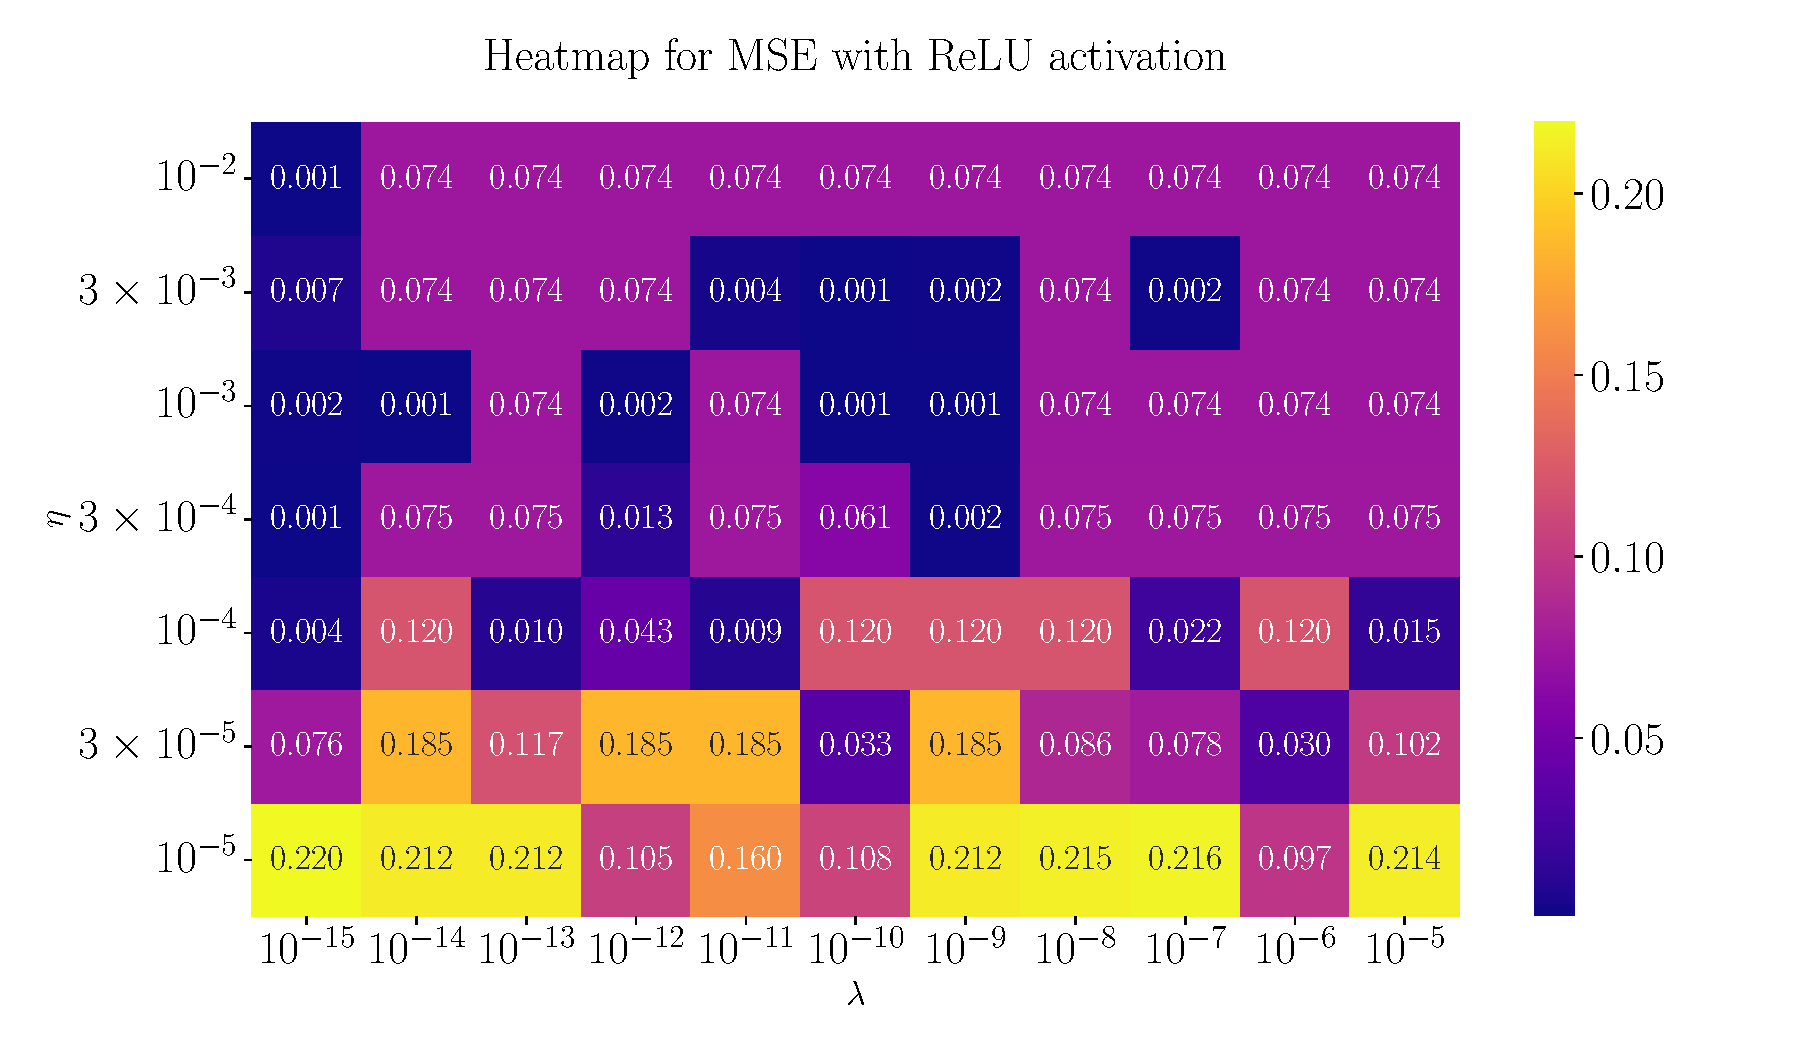
\includegraphics[width=\textwidth]{Python/Figures/Heatmap_MSE_ReLU_Franke_Epochs250.pdf}
		\caption{ReLU}
	\end{subfigure}
	\hfill
	\begin{subfigure}{0.4353\textwidth}
		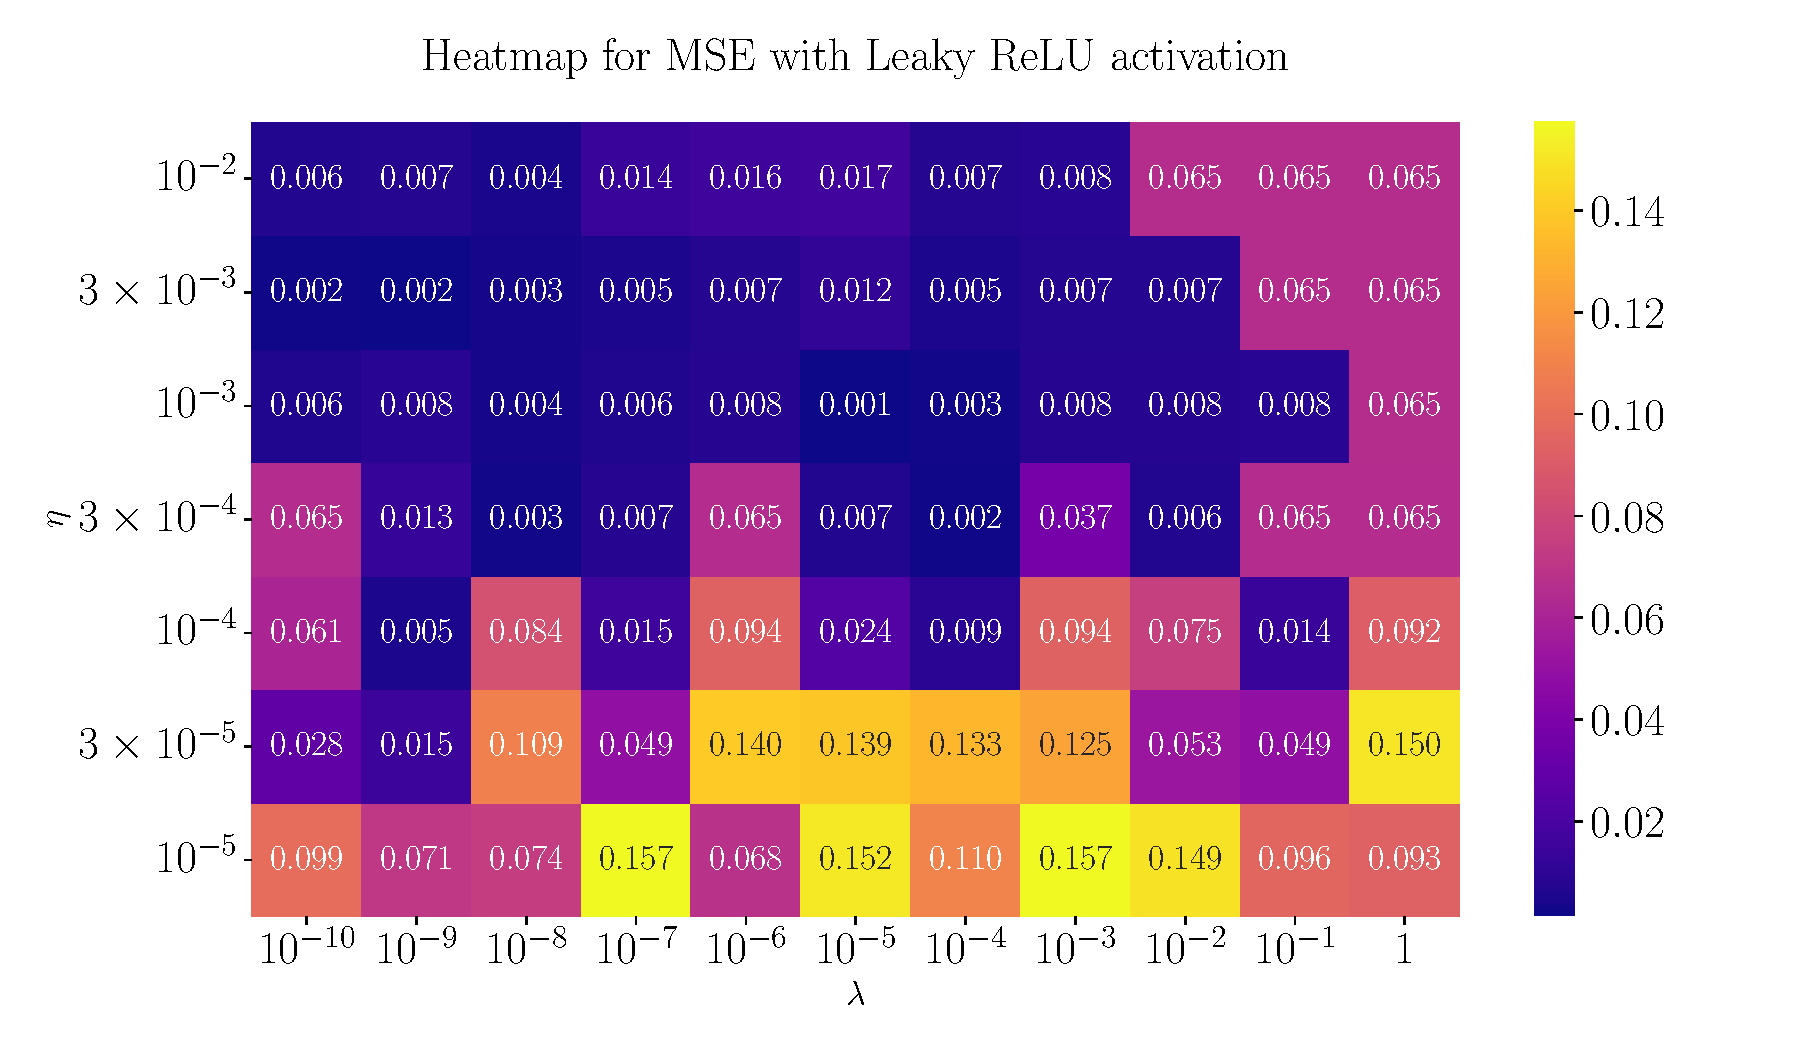
\includegraphics[width=\textwidth]{Python/Figures/Heatmap_MSE_Leaky ReLU_Franke_Epochs250.pdf}
		\caption{LReLU}
	\end{subfigure}
	\hfill\newline
	\begin{subfigure}{0.4353\textwidth}
		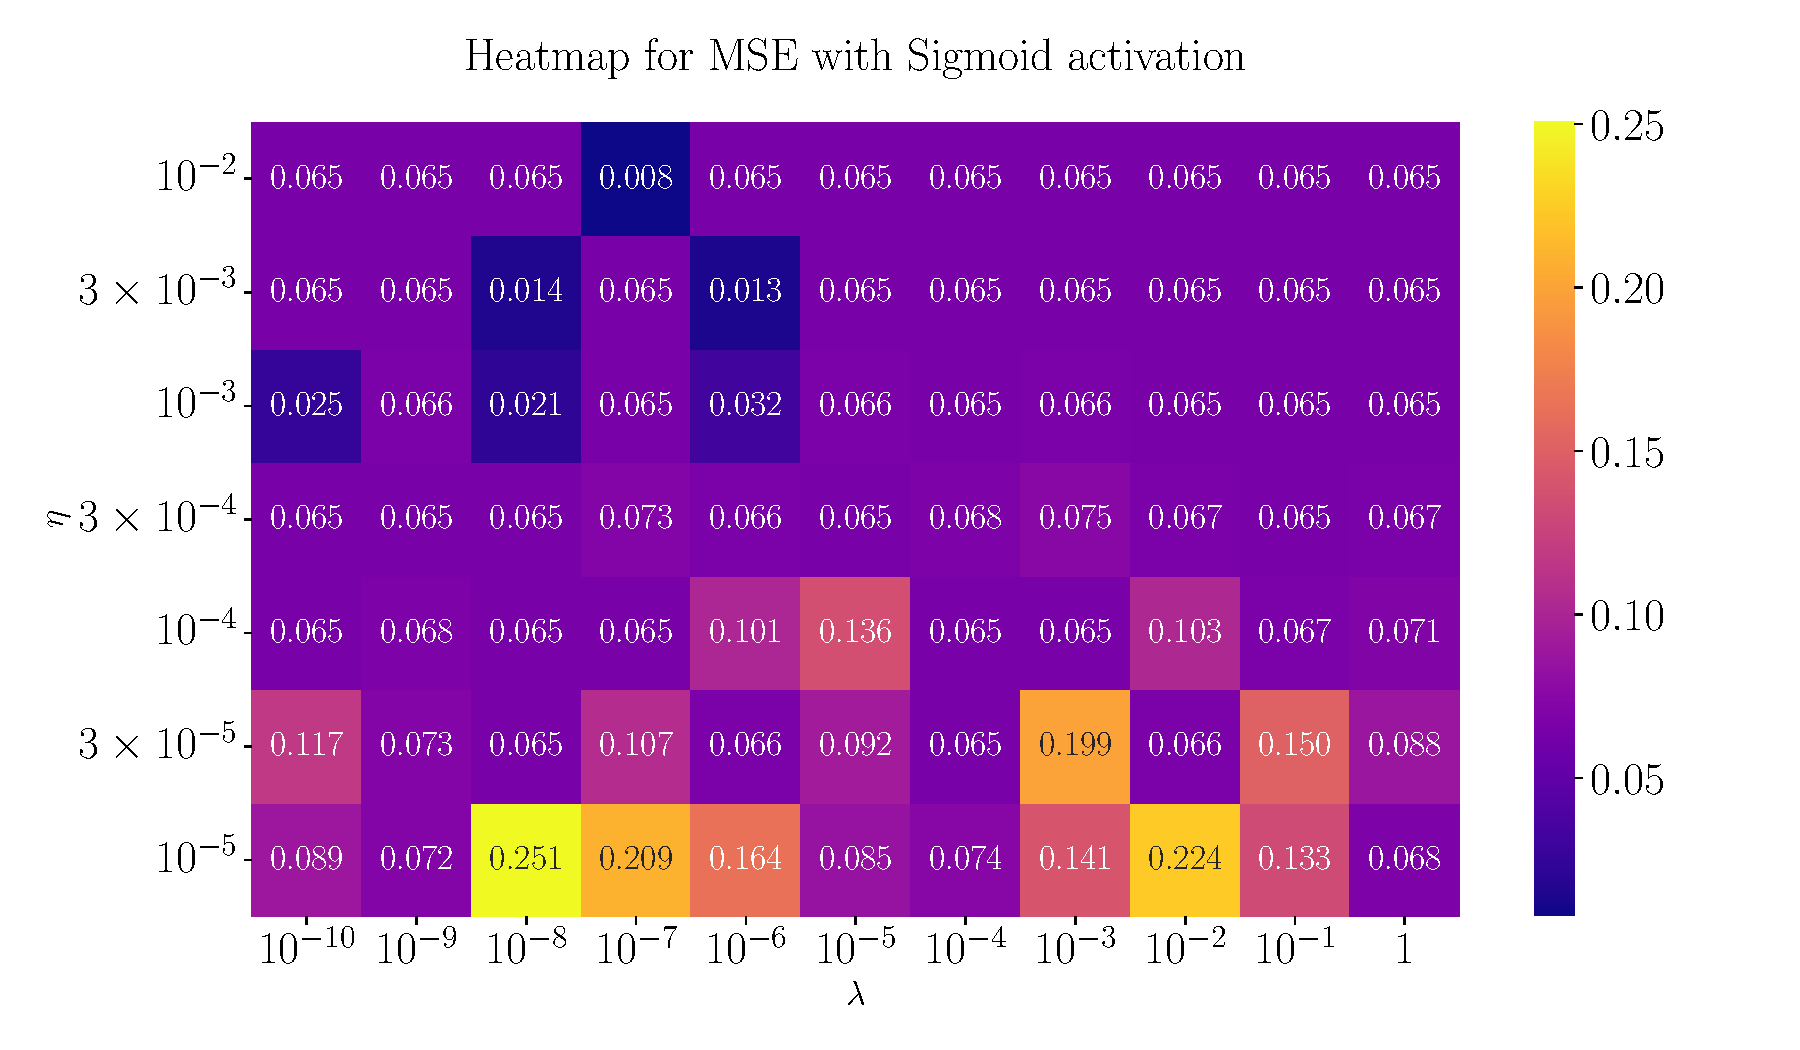
\includegraphics[width=\textwidth]{Python/Figures/Heatmap_MSE_Sigmoid_Franke_Epochs250.pdf}
		\caption{Sigmoid}
	\end{subfigure}
	\caption{MSE for various combinations of $\eta$ and $\lambda$ for ReLU, LReLU and Sigmoid activation functions with $250$ epochs on the Franke function.}
	\label{fig:FFNN_Franke_heatmaps}	
\end{figure*}
\begin{figure*}[ht!]
	\begin{subfigure}{0.4353\textwidth}
		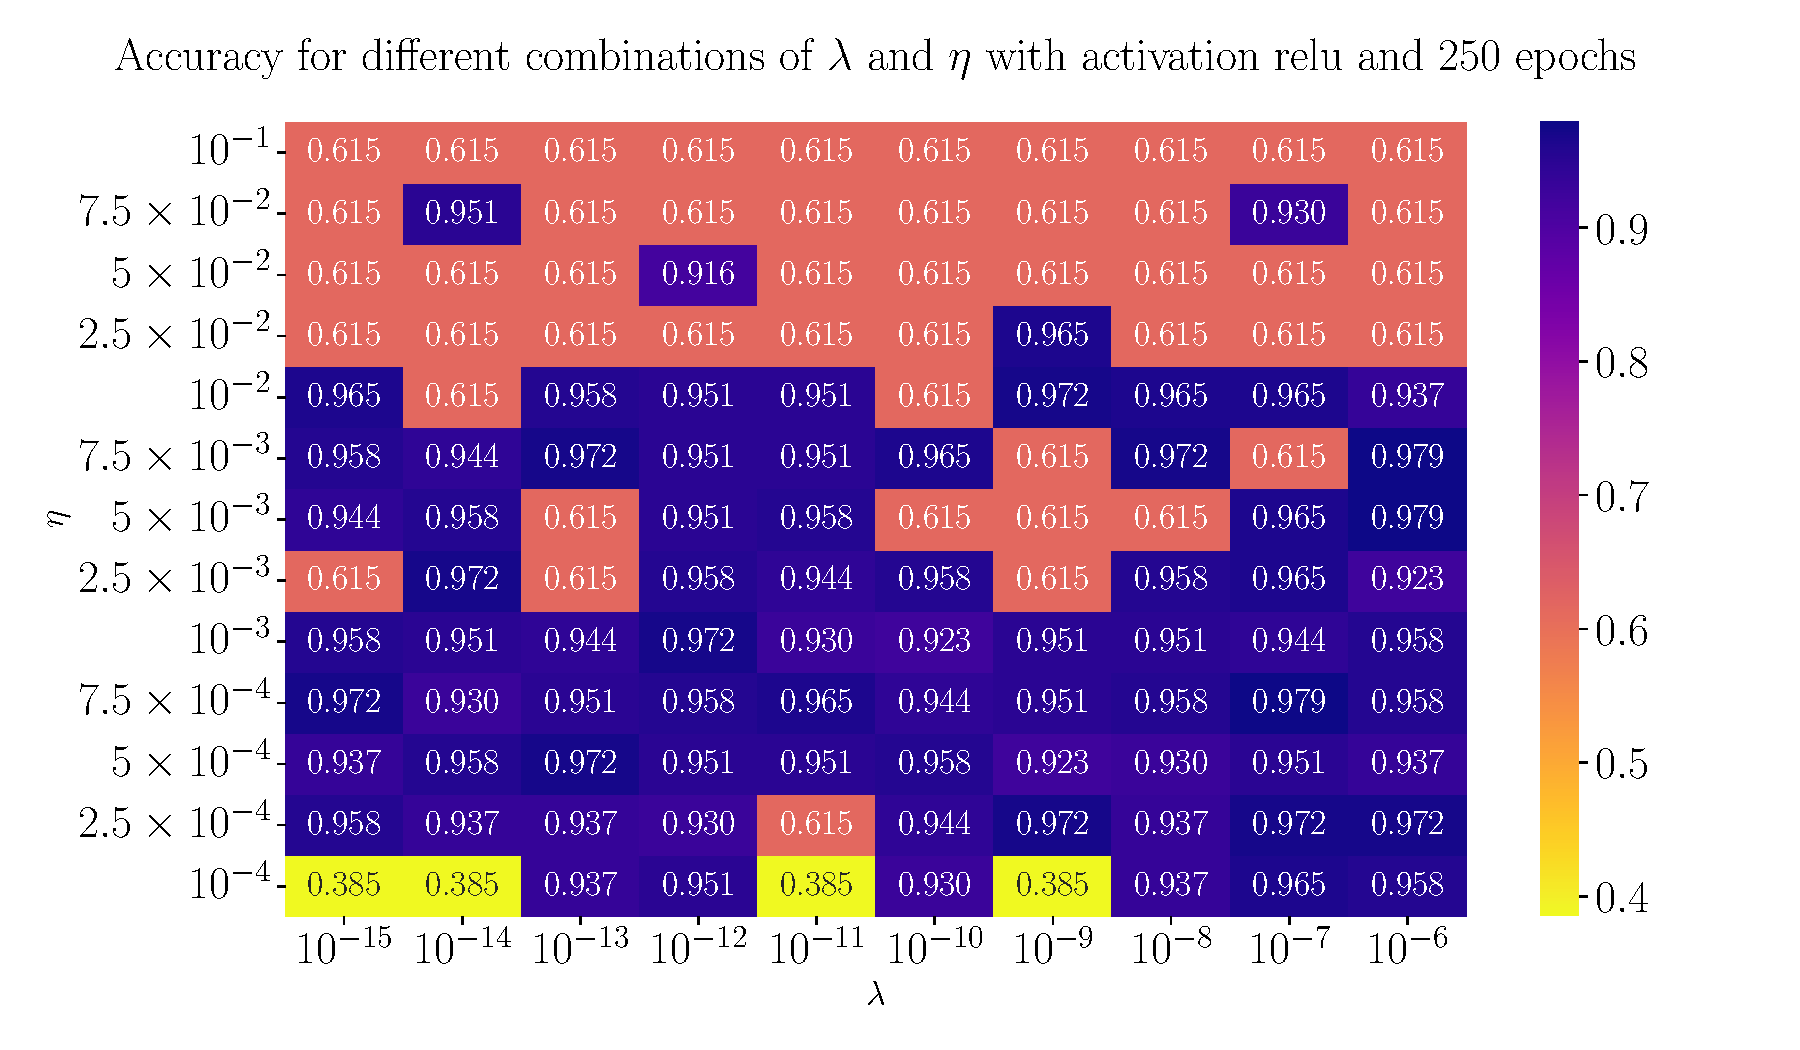
\includegraphics[width=\textwidth]{Python/Figures/Cancer_Accuracy_Heatmap_relu_Epochs250.pdf}
		\caption{ReLU}
		\label{fig:ReLU_heatmap}
	\end{subfigure}
	\hfill
	\begin{subfigure}{0.4353\textwidth}
		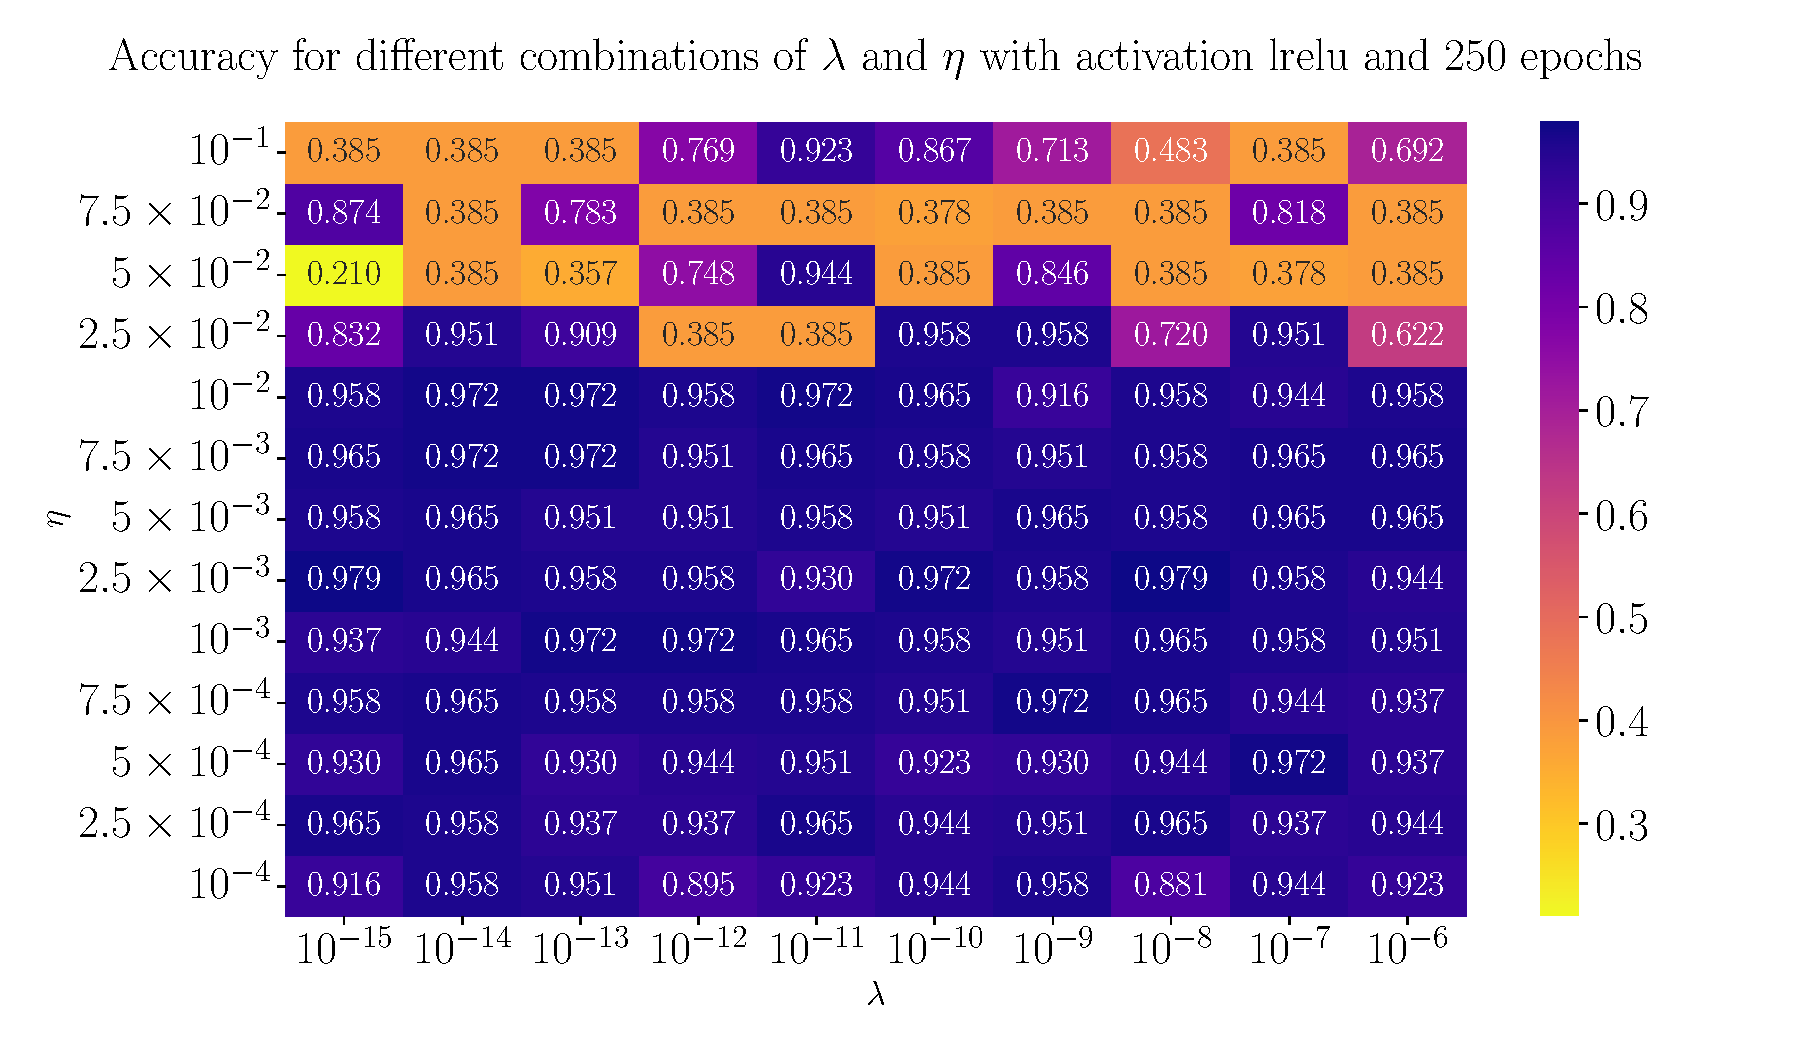
\includegraphics[width=\textwidth]{Python/Figures/Cancer_Accuracy_Heatmap_lrelu_Epochs250.pdf}
		\caption{LReLU}
		\label{fig:LReLU_heatmap}
	\end{subfigure}
	\hfill\newline
	\begin{subfigure}{0.4353\textwidth}
		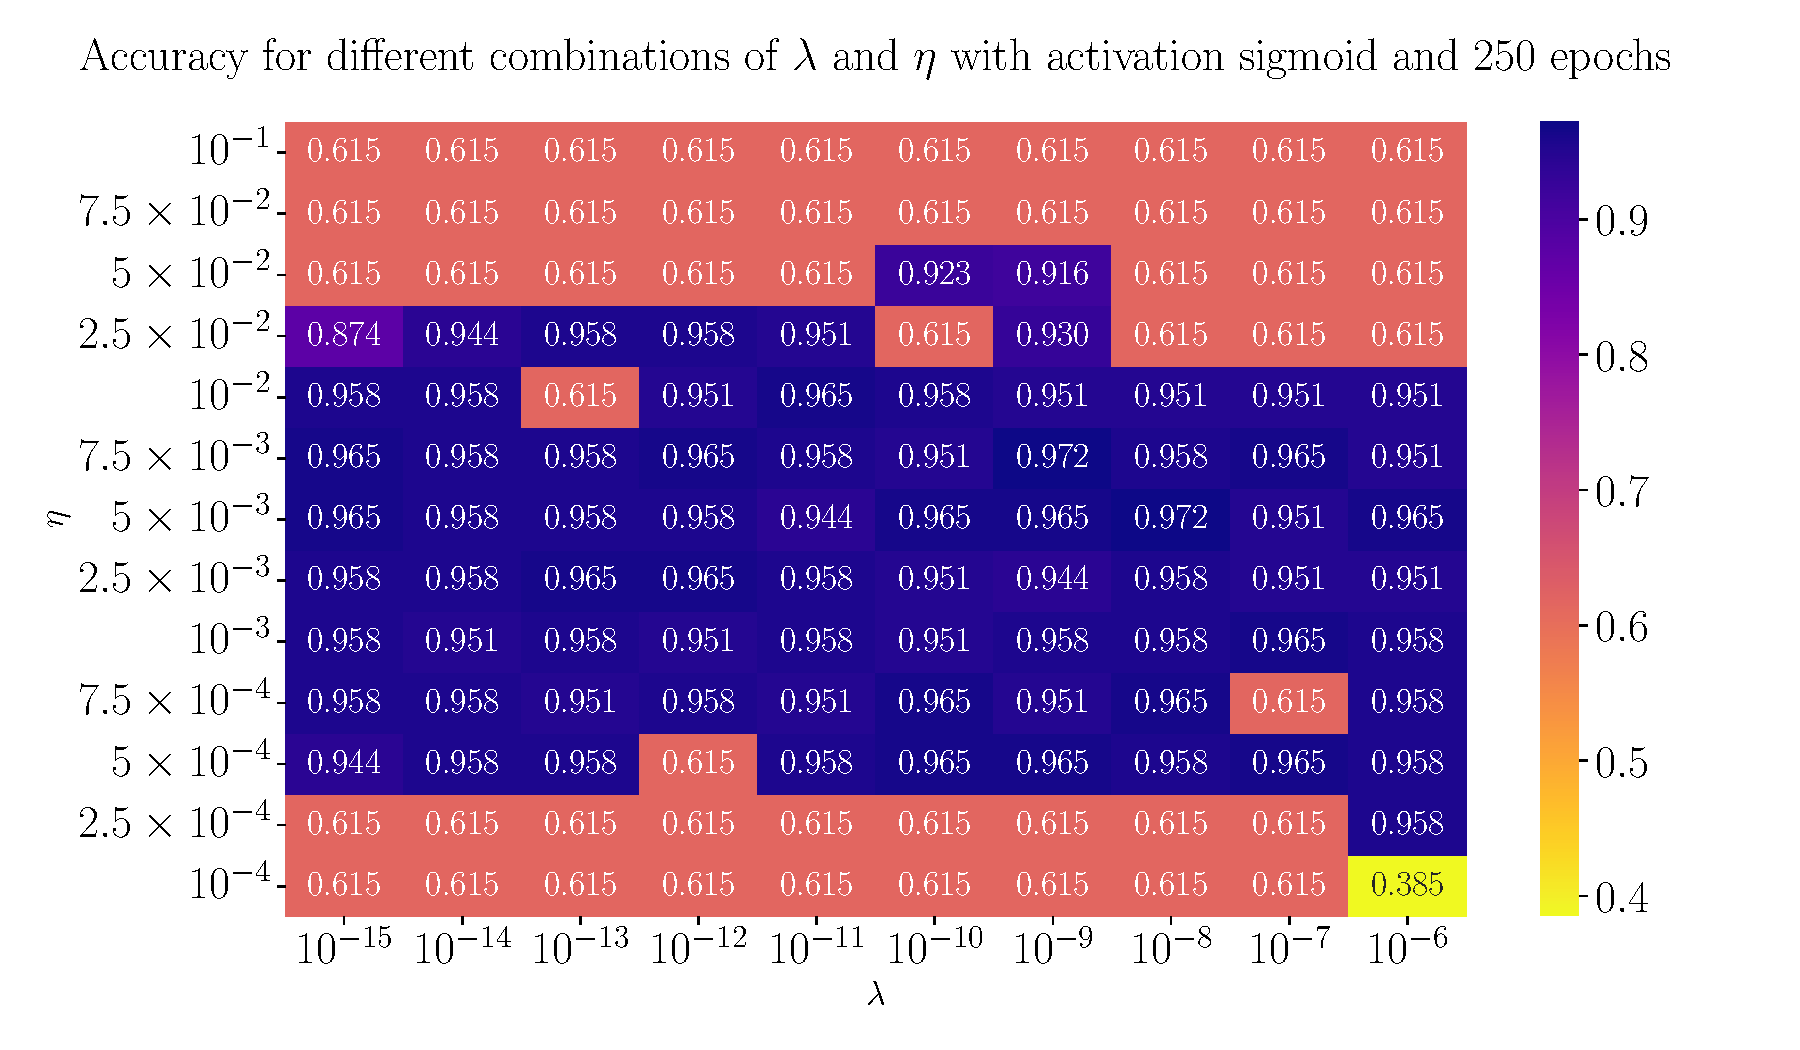
\includegraphics[width=\textwidth]{Python/Figures/Cancer_Accuracy_Heatmap_sigmoid_Epochs250.pdf}
		\caption{Sigmoid}
		\label{fig:Sigmoid_heatmap}
	\end{subfigure}
	\caption{Accuracy for various combinations of $\eta$ and $\lambda$ for ReLU, LReLU and Sigmoid activation functions with $250$ epochs on the breast cancer dataset.}
	\label{fig:FFNN_cancer_heatmaps}
\end{figure*}

	
\end{document}